\section{各サブシステムのフローチャート}
各サブシステムのフローチャートを示します。

\subsection{アカウント作成システム(学生用)}
アカウント作成システム(学生用)では、学生がアカウント新規登録画面にて情報を入力し、登録ボタンを押下することで処理が行われます。
アカウント作成システム(学生用)のシーケンス図とフローチャートを以下に示します。

\begin{figure}[htbp]
  \begin{center}
    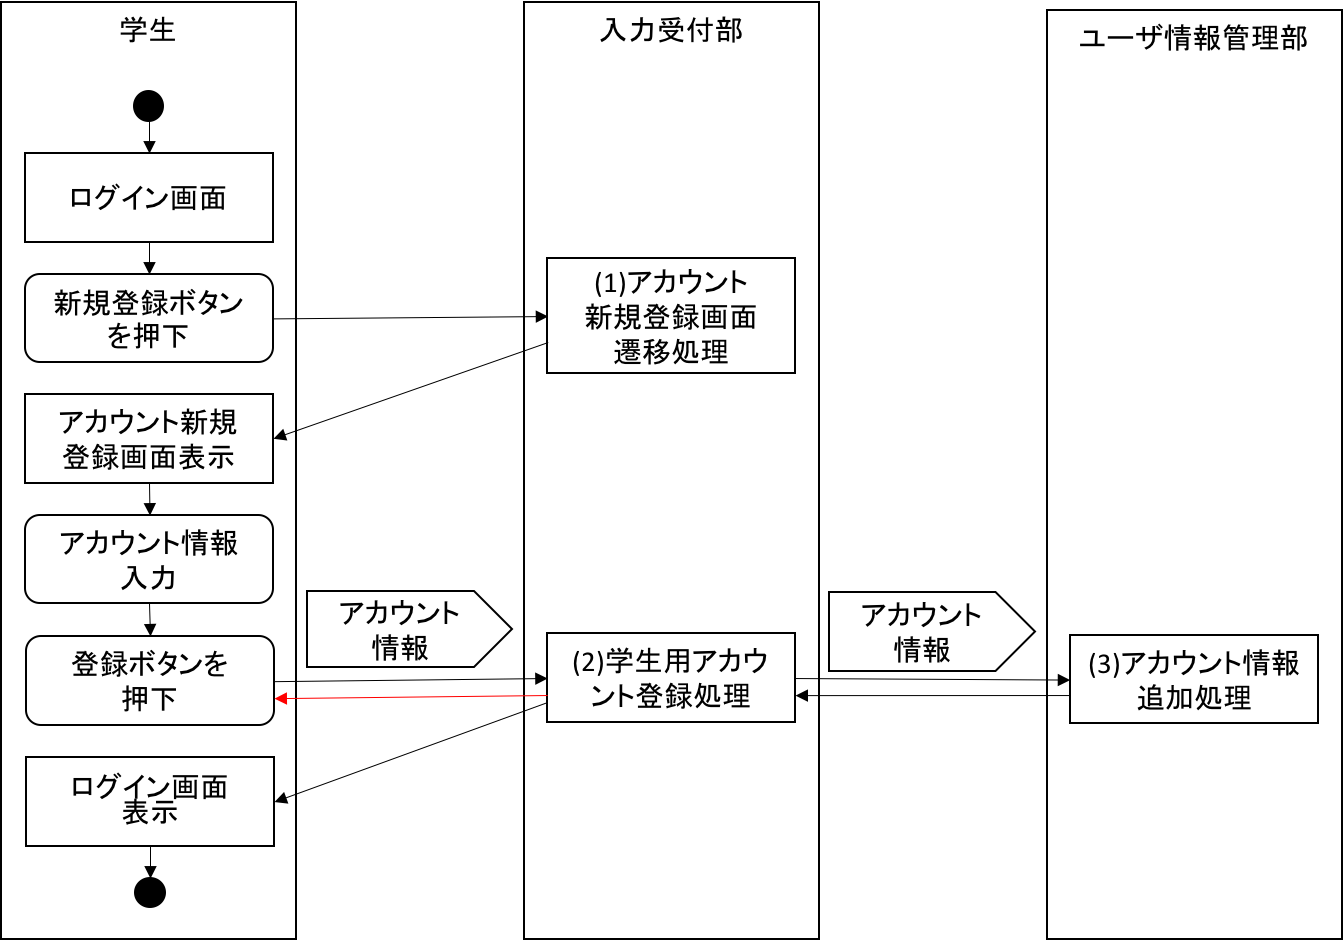
\includegraphics[width=1\linewidth,clip]{./img/seq1}
    \caption{アカウント作成システム(学生用)のシーケンス図}\label{fig:seq1}
  \end{center}
\end{figure}

(1)は、新規登録ボタンを押下することでアカウント新規登録画面へ遷移する処理です。\\
(2)・(3)は、学生用アカウントを登録する処理です。


\begin{figure}[htbp]
 \begin{minipage}{0.5\hsize}
  \begin{center}
   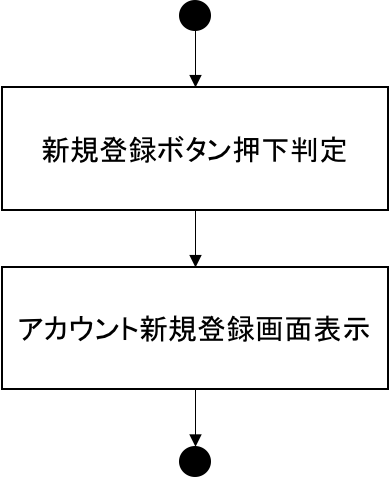
\includegraphics[width=0.5\linewidth,clip]{./img/flow/1.png}
  \end{center}
 \end{minipage}
 \begin{minipage}{0.5\hsize}
  \begin{center}
   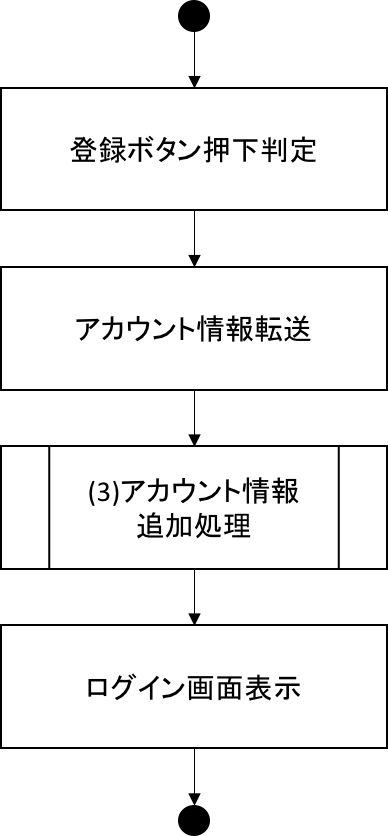
\includegraphics[width=0.5\linewidth,clip]{./img/flow/2.png}
  \end{center}
 \end{minipage}
 \caption{左:(1)のフローチャート 右:(2)のフローチャート}\label{fig:1to2}
\end{figure}

\begin{figure}[htbp]
  \begin{center}
    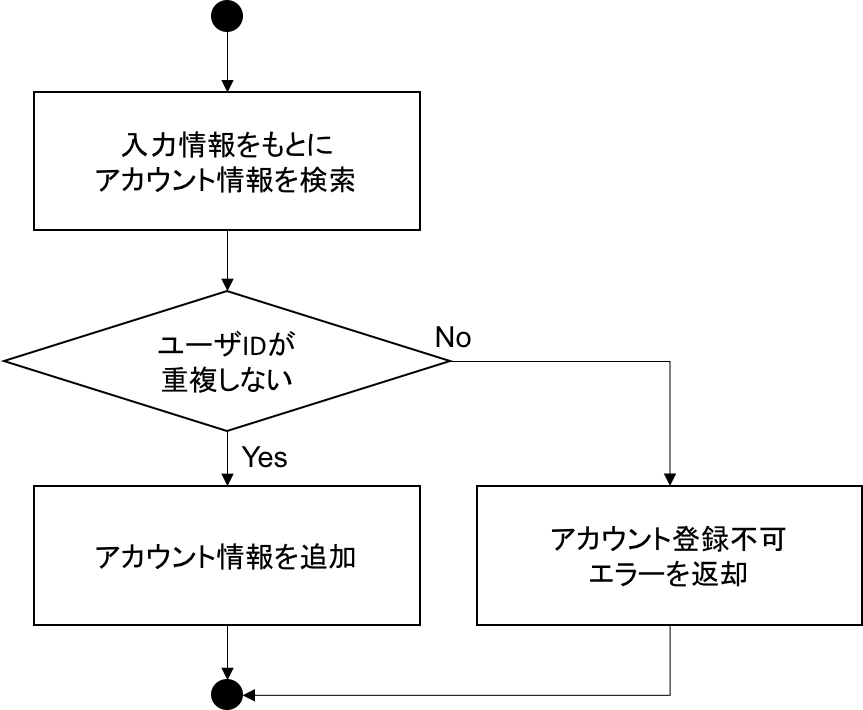
\includegraphics[width=0.7\linewidth,clip]{./img/flow/3.png}
    \caption{(3)のフローチャート}\label{fig:3}
  \end{center}
\end{figure}




\clearpage




\subsection{アカウント作成システム(管理者用)}
アカウント作成システム(管理者用)では、他のアカウント新規登録画面にてアカウント情報を入力し、登録ボタンを押下することで処理が行われます。
アカウント作成システム(管理者用)のシーケンス図とフローチャートを以下に示します。

\begin{figure}[htbp]
  \begin{center}
    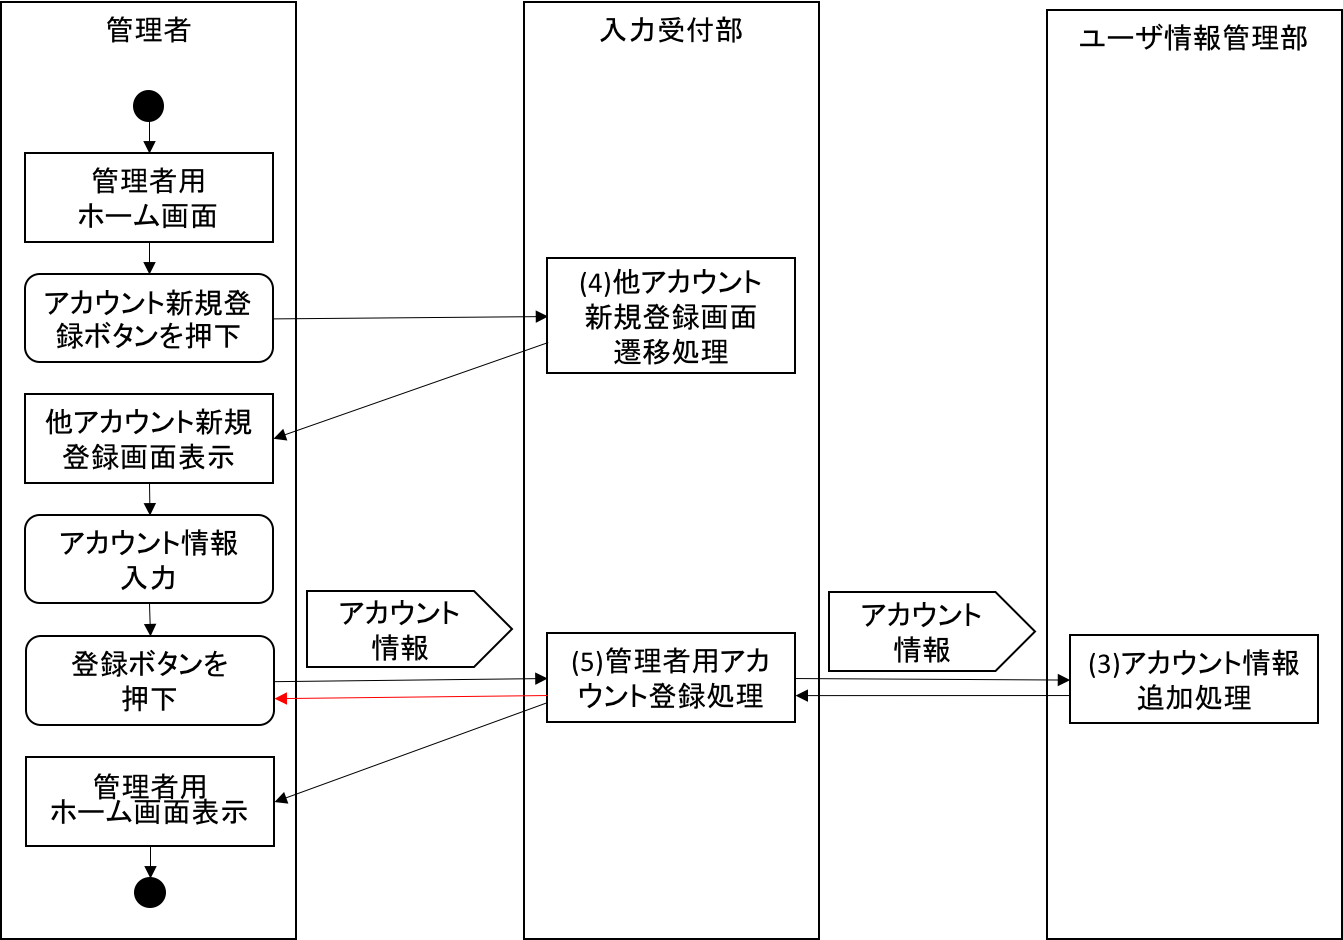
\includegraphics[width=1\linewidth,clip]{./img/seq2.png}
    \caption{アカウント作成システム(管理者用)のシーケンス図}\label{fig:seq2}
  \end{center}
\end{figure}

(4)は、他のアカウント新規登録画面へ遷移する処理です。\\
(5)は、登録ボタンを押下することで新規アカウントを作成する処理です。


\begin{figure}[htbp]
 \begin{minipage}{0.5\hsize}
  \begin{center}
   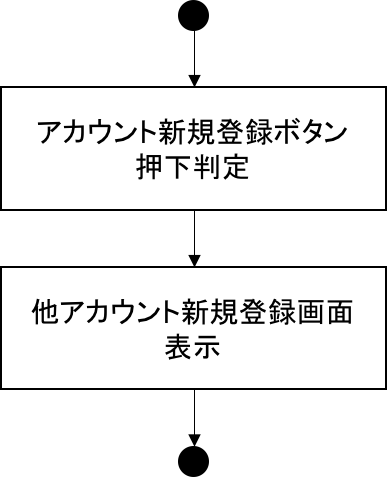
\includegraphics[width=0.6\linewidth,clip]{./img/flow/4.png}
  \end{center}
 \end{minipage}
 \begin{minipage}{0.5\hsize}
  \begin{center}
   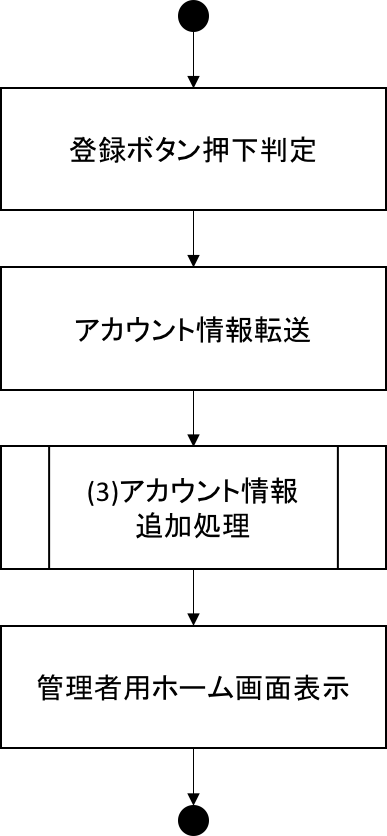
\includegraphics[width=0.5\linewidth,clip]{./img/flow/5.png}
  \end{center}
 \end{minipage}
 \caption{左:(4)のフローチャート 右:(5)のフローチャート}\label{fig:4to5}
\end{figure}


\clearpage
\subsection{アカウント情報編集システム}
アカウント情報編集システムでは、登録情報編集画面にて情報を変更し、変更ボタンを押下することで処理が行われます。
アカウント情報編集システムのシーケンス図とフローチャートを以下に示します。

\begin{figure}[htbp]
  \begin{center}
    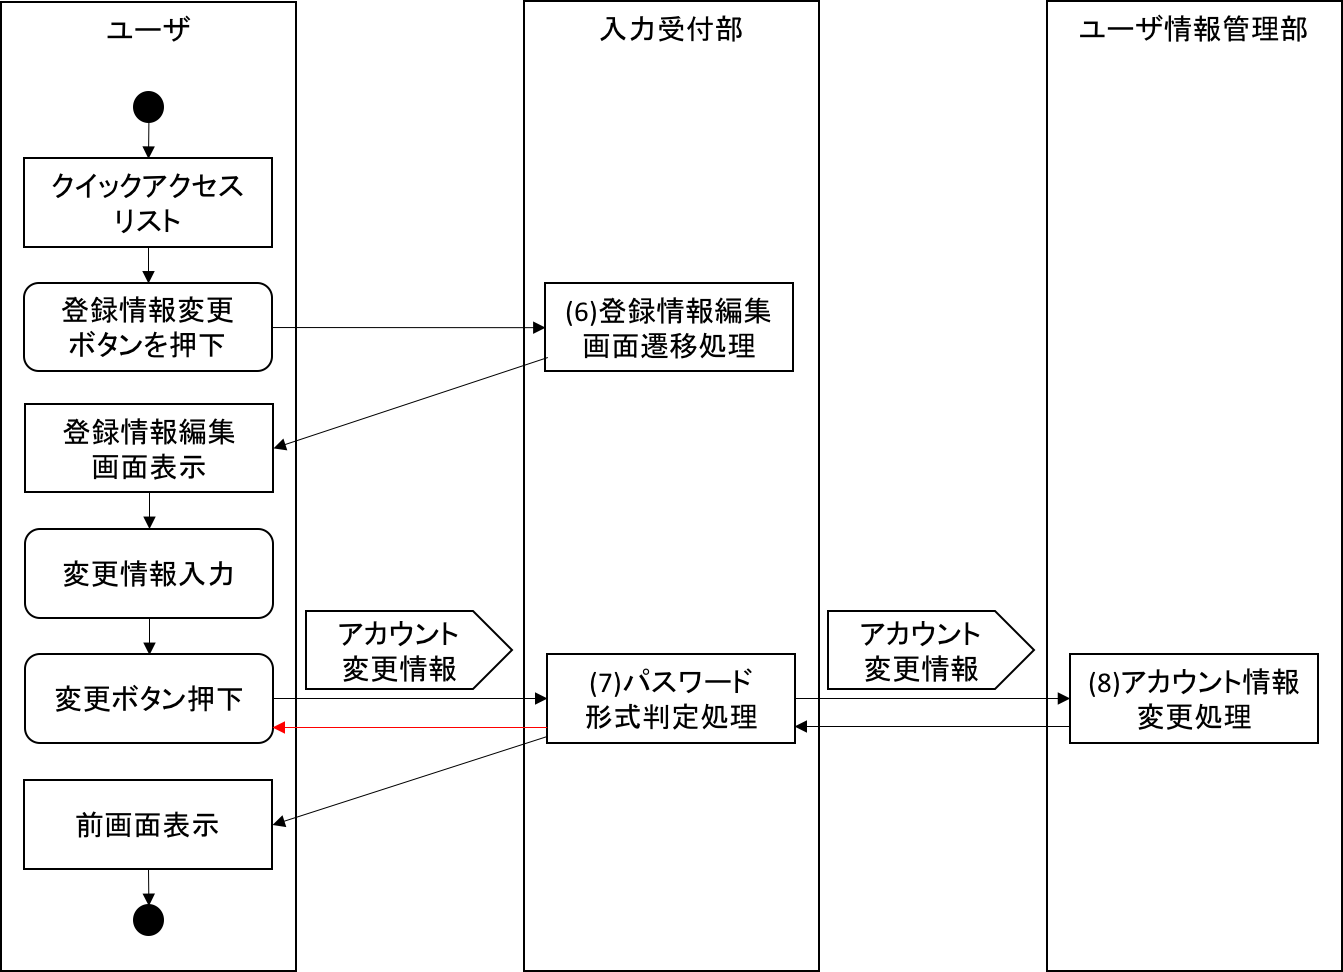
\includegraphics[width=1\linewidth,clip]{./img/seq3.png}
    \caption{アカウント情報編集システムのシーケンス図}\label{fig:seq3}
  \end{center}
\end{figure}

(6)は、登録情報編集画面へ遷移する処理です。\\
(7)・(8)は、変更情報を入力し変更ボタンを押下することで、登録情報の変更を行う処理です。

\begin{figure}[htbp]
 \begin{minipage}{0.5\hsize}
  \begin{center}
   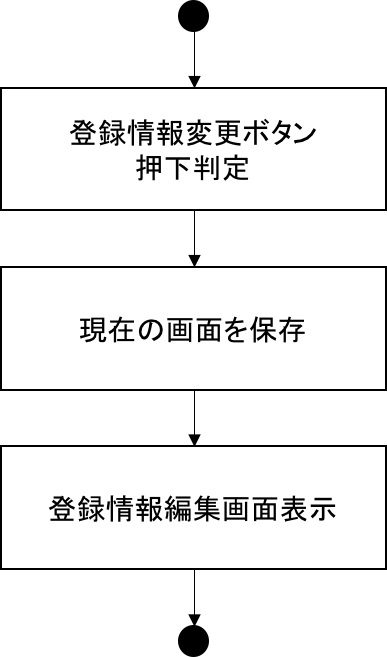
\includegraphics[width=0.5\linewidth,clip]{./img/flow/6.png}
  \end{center}
 \end{minipage}
 \begin{minipage}{0.5\hsize}
  \begin{center}
   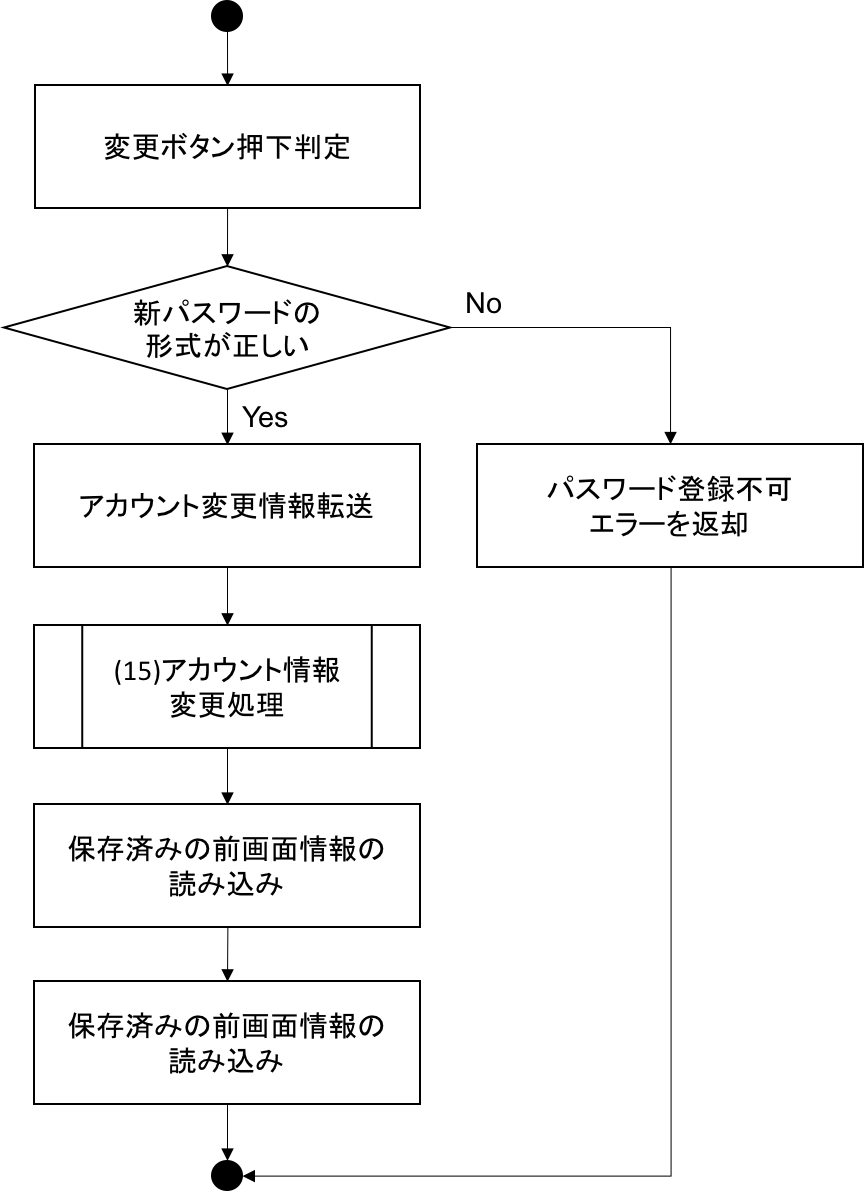
\includegraphics[width=1\linewidth,clip]{./img/flow/7.png}
  \end{center}
 \end{minipage}
 \caption{左:(6)のフローチャート 右:(7)のフローチャート}\label{fig:6to7}
\end{figure}

\begin{figure}[htbp]
  \begin{center}
    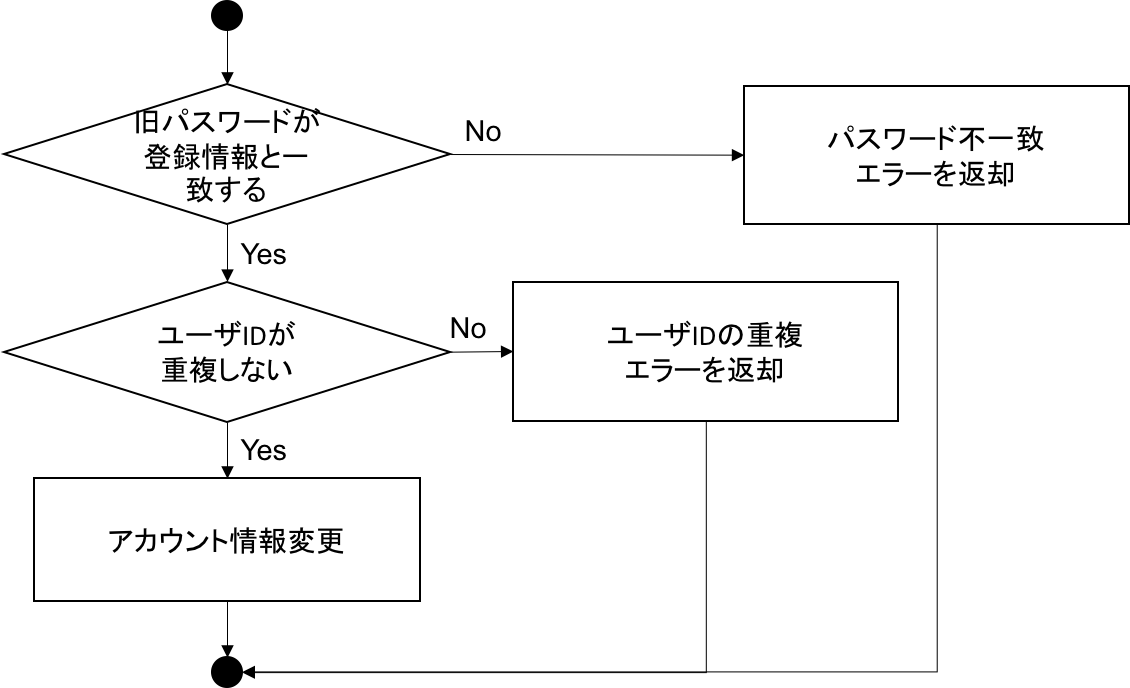
\includegraphics[width=0.75\linewidth,clip]{./img/flow/8.png}
    \caption{(8)のフローチャート}\label{fig:8}
  \end{center}
\end{figure}


\clearpage
\subsection{アカウント削除システム}
アカウント削除システムでは、登録から指定年数が経ったアカウントを削除する処理を行います。
アカウント削除システムのシーケンス図とフローチャートを以下に示します。

\begin{figure}[htbp]
  \begin{center}
    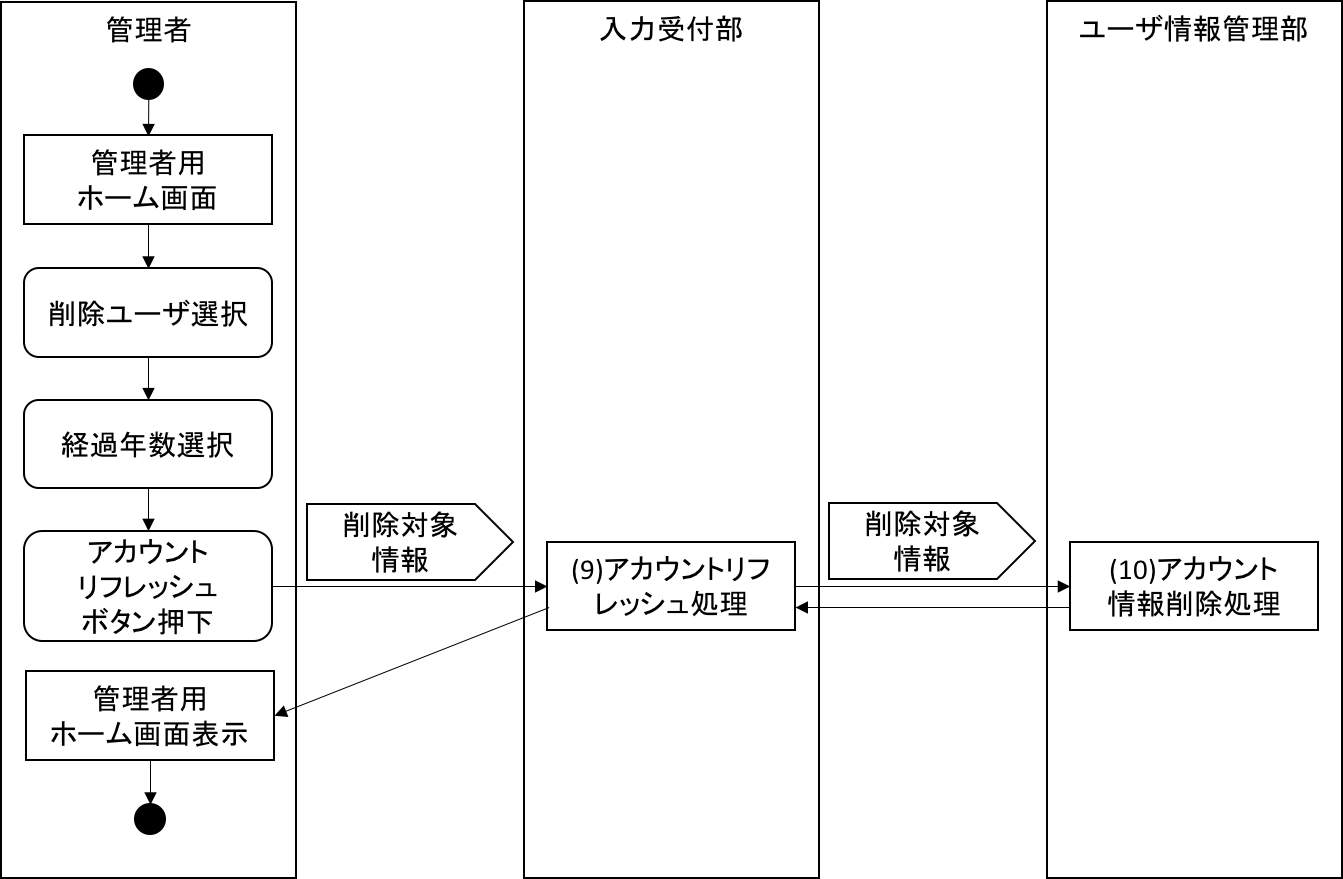
\includegraphics[width=1\linewidth,clip]{./img/seq4.png}
    \caption{アカウント削除システムのシーケンス図}\label{fig:seq4}
  \end{center}
\end{figure}

(9)・(10)は、登録から指定年数を過ぎたアカウントを一斉に削除する処理です。

\begin{figure}[htbp]
 \begin{minipage}{0.5\hsize}
  \begin{center}
   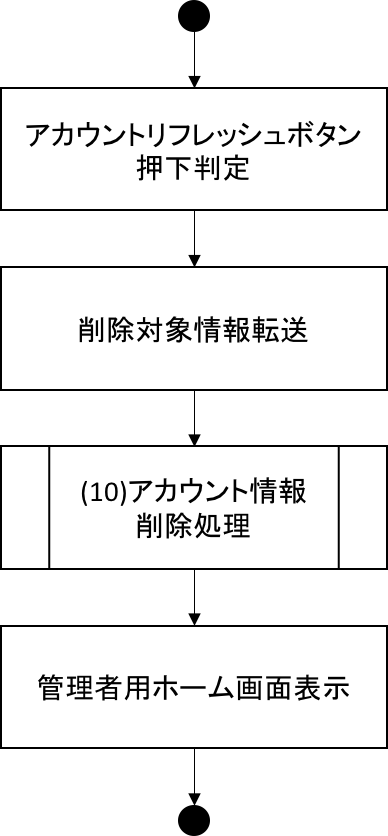
\includegraphics[width=0.5\linewidth,clip]{./img/flow/9.png}
  \end{center}
 \end{minipage}
 \begin{minipage}{0.5\hsize}
  \begin{center}
   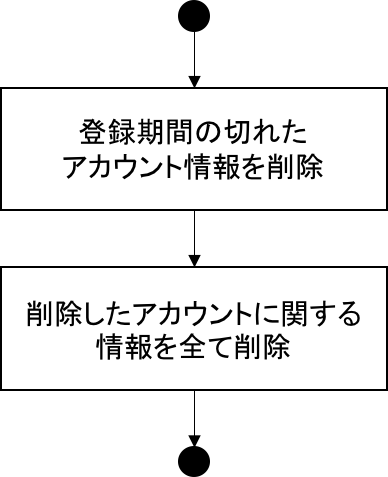
\includegraphics[width=0.5\linewidth,clip]{./img/flow/10.png}
  \end{center}
 \end{minipage}
 \caption{左:(9)のフローチャート 右:(10)のフローチャート}\label{fig:9to10}
\end{figure}



\clearpage

\subsection{ログインシステム(学生用)}
ログインシステム(学生用)では、学生がログイン画面においてユーザ情報を入力し、ログインボタンを押下することによって処理が行われます。
ログインシステム(学生用)のシーケンス図とフローチャートを以下に示します。

\begin{figure}[htbp]
  \begin{center}
    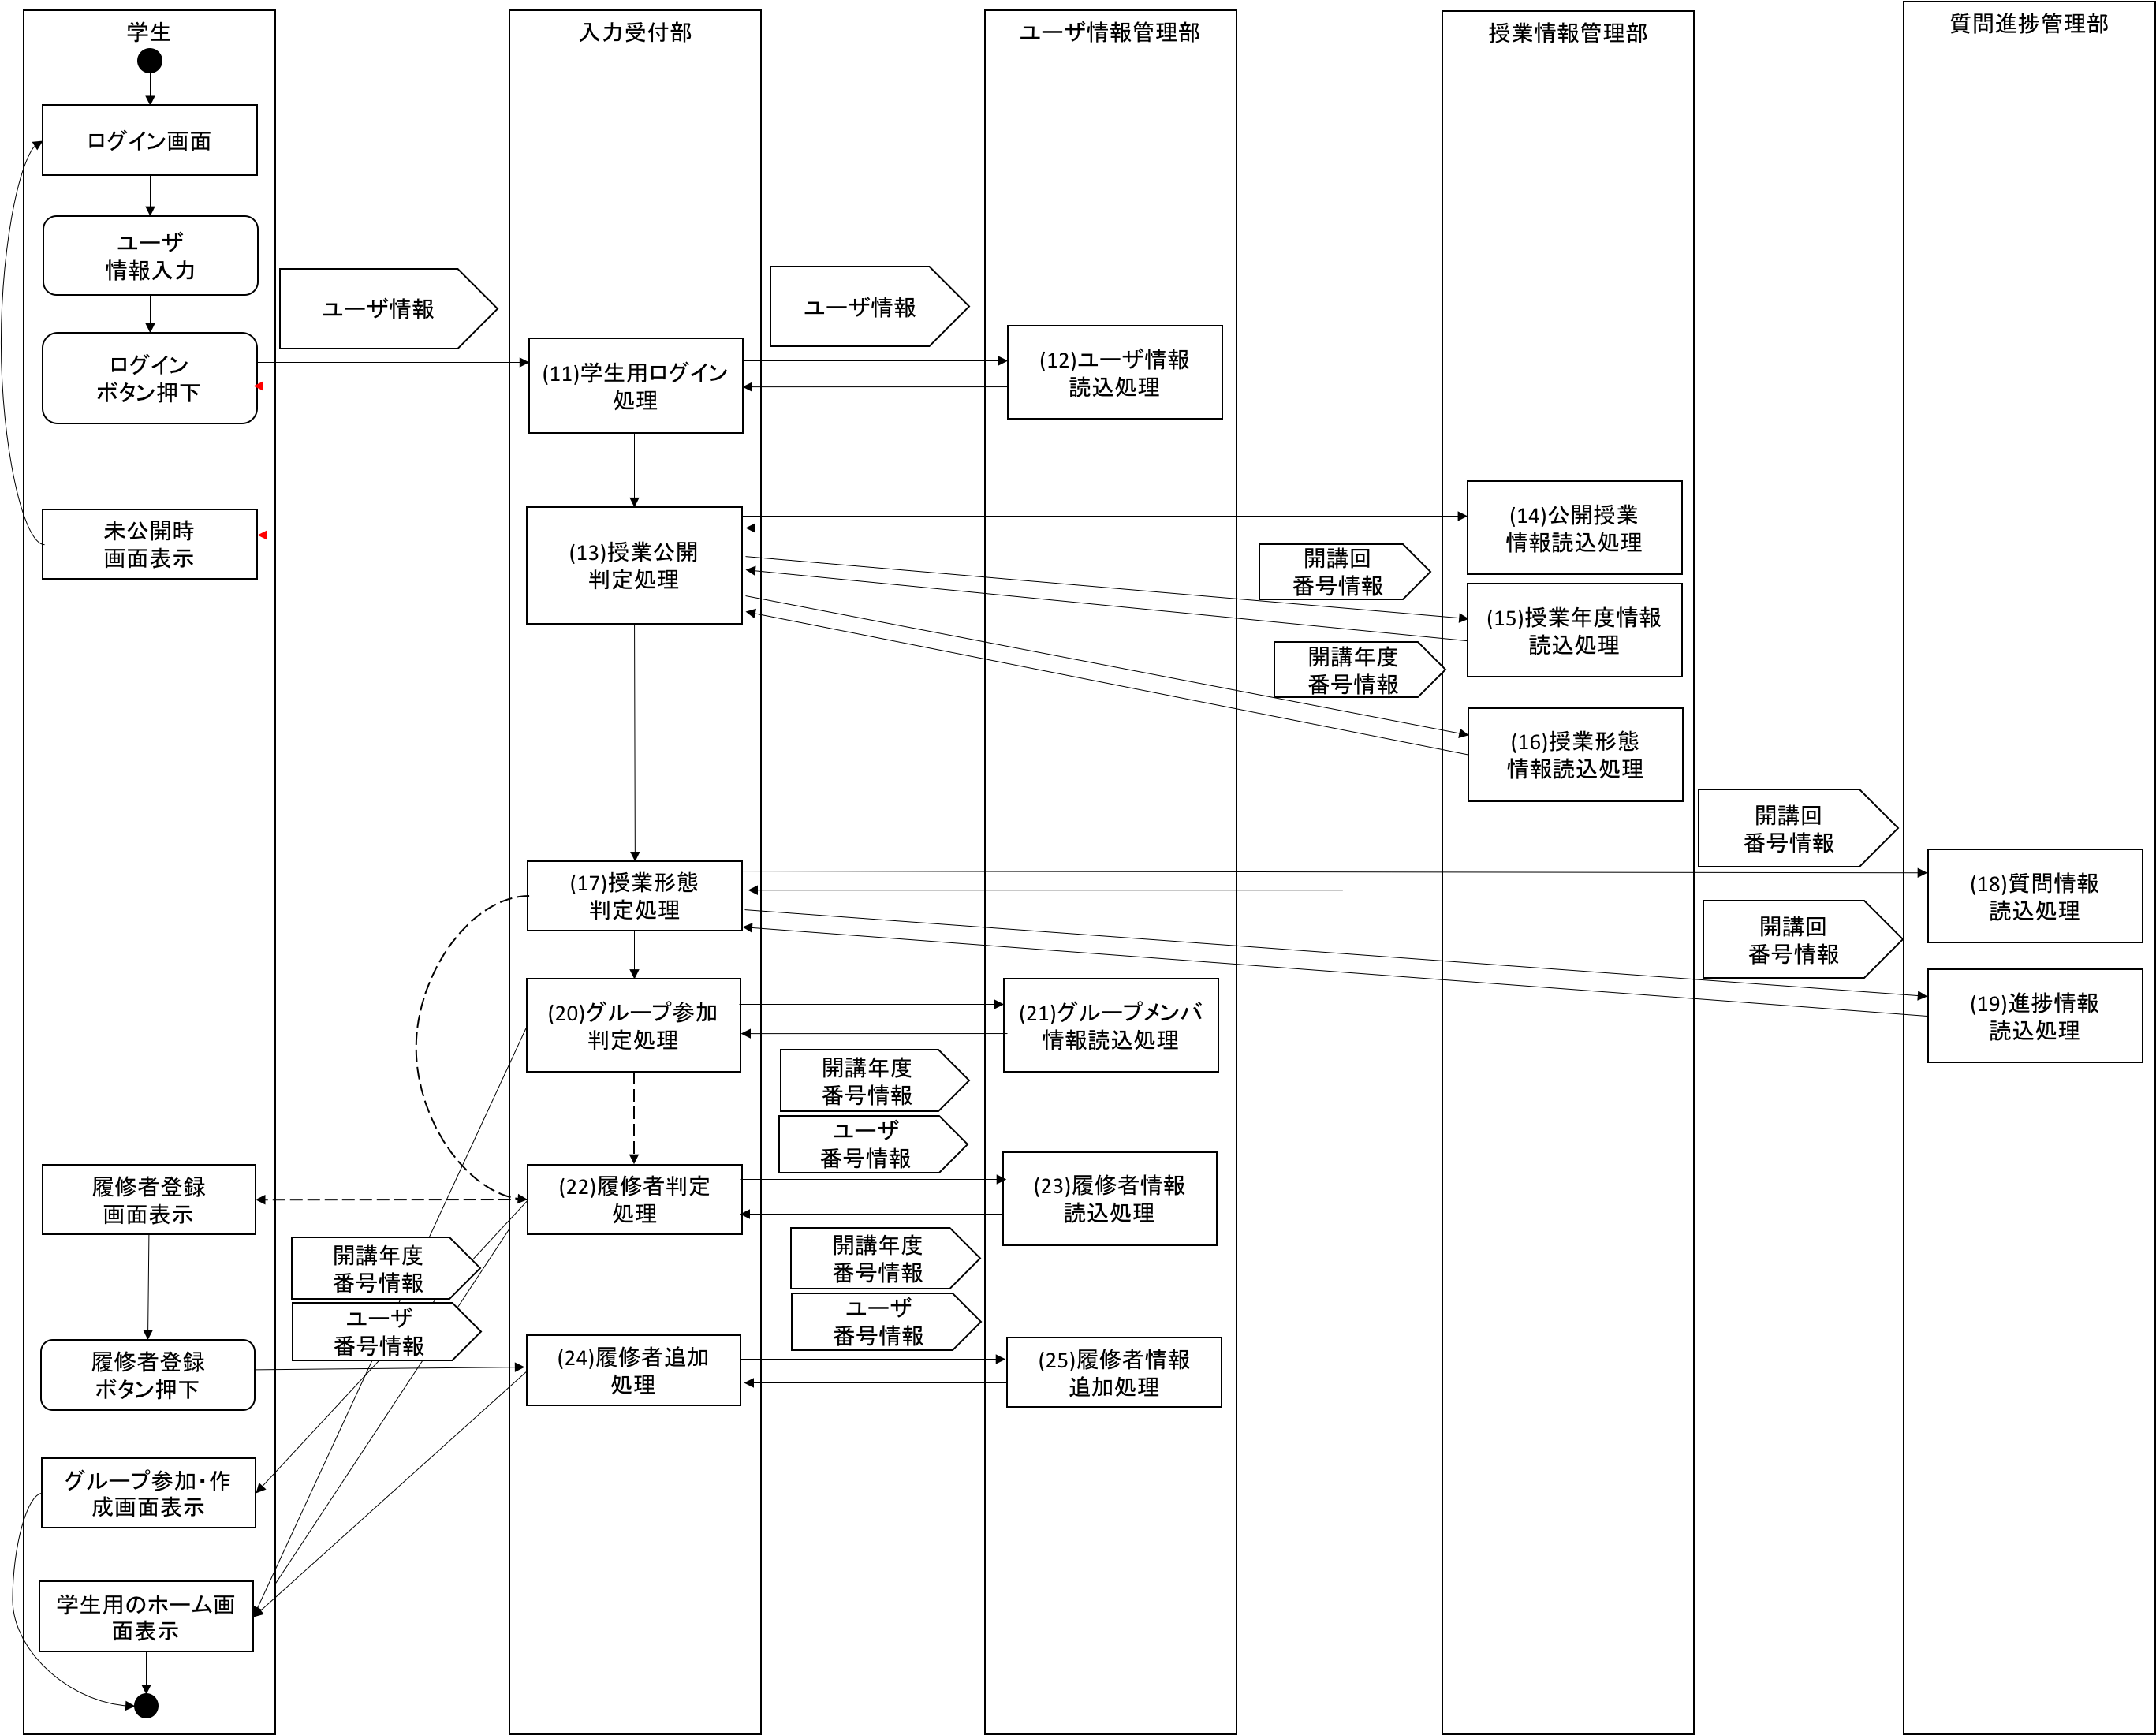
\includegraphics[width=1\linewidth,clip]{./img/seq5.png}
    \caption{ログインシステム(学生用)のシーケンス図}\label{fig:seq5}
  \end{center}
\end{figure}

(11)・(12)は、ログイン可能かどうかの判定を行う処理です。\\
また、入力されたユーザ情報が学生のものであるかの判定を行います。\\
(13)~(16)は、現在授業が公開されているかの判定を行う処理です。\\
授業が公開されている場合は、何の授業が公開されているかの識別を行います。\\
(17)~(19)は、公開されている授業がグループワークなのか、また、進捗機能を用いるかの判定を行う処理です。\\
(20)・(21)は、ユーザがグループに参加しているかの判定を行う処理です。\\
(22)・(23)は、ユーザが履修者として登録されているかどうかの判定を行う処理です。\\
(24)・(25)は、ユーザを履修者として登録する処理です。

\begin{figure}[htbp]
 \begin{minipage}{0.5\hsize}
  \begin{center}
   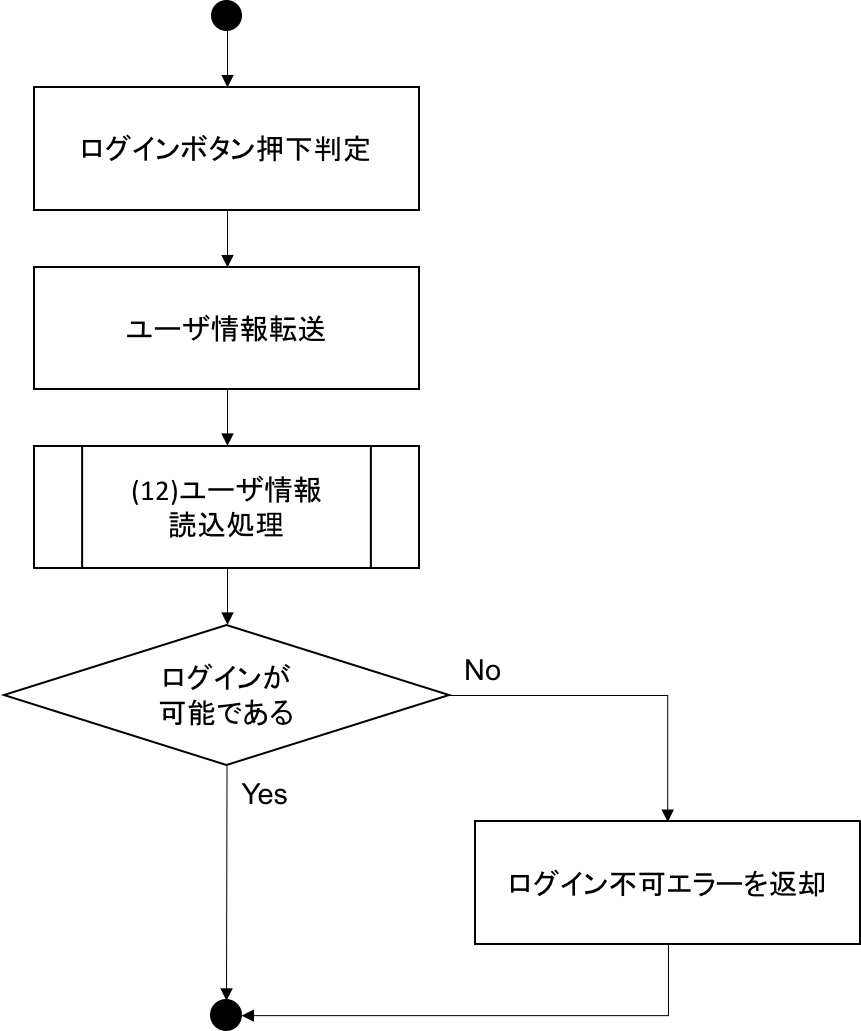
\includegraphics[width=0.9\linewidth,clip]{./img/flow/11.png}
  \end{center}
 \end{minipage}
 \begin{minipage}{0.5\hsize}
  \begin{center}
   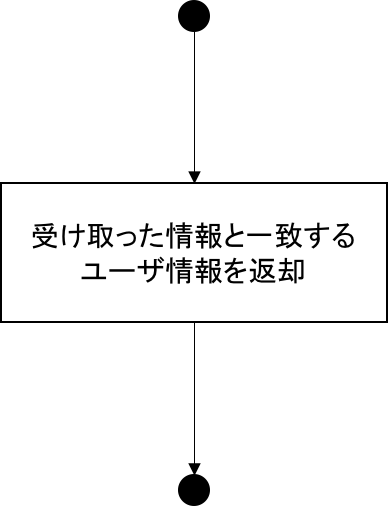
\includegraphics[width=0.5\linewidth,clip]{./img/flow/12.png}
  \end{center}
 \end{minipage}
 \caption{左:(11)のフローチャート 右:(12)のフローチャート}\label{fig:11to12}
\end{figure}

\begin{figure}[htbp]
  \begin{center}
    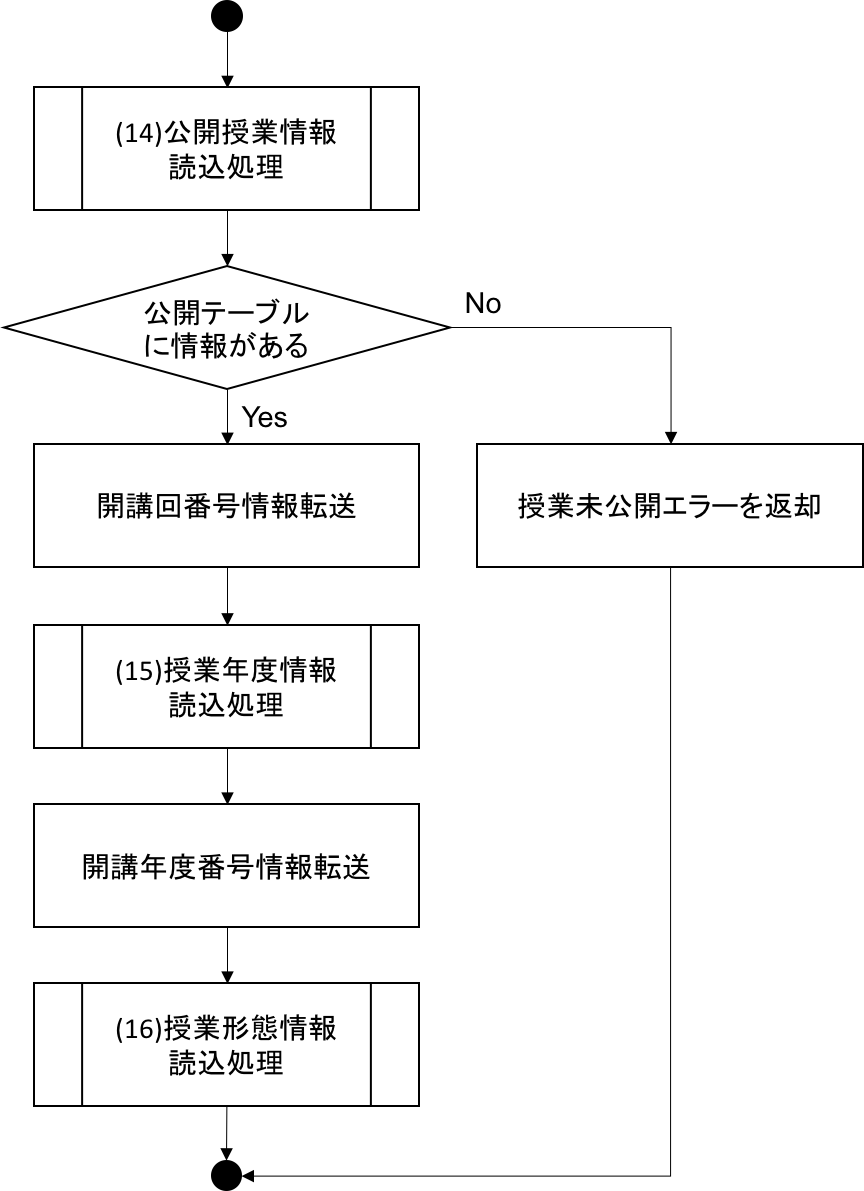
\includegraphics[width=0.5\linewidth,clip]{./img/flow/13.png}
    \caption{(13)のフローチャート}\label{fig:13}
  \end{center}
\end{figure}



\begin{figure}[htbp]
  \begin{tabular}{c}
 \begin{minipage}{0.33\hsize}
  \begin{center}
   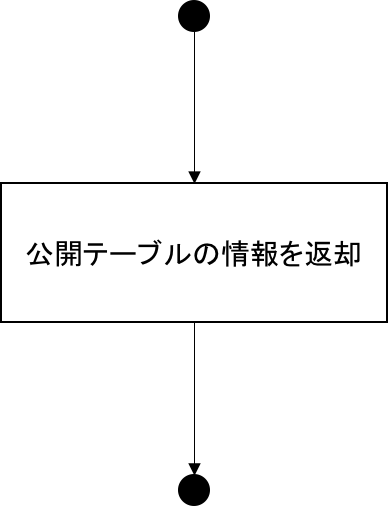
\includegraphics[width=0.8\linewidth,clip]{./img/flow/14.png}
  \end{center}
 \end{minipage}
 \begin{minipage}{0.33\hsize}
  \begin{center}
   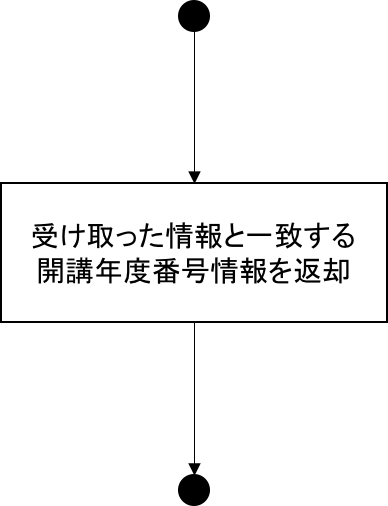
\includegraphics[width=0.8\linewidth,clip]{./img/flow/15.png}
  \end{center}
 \end{minipage}
 \begin{minipage}{0.33\hsize}
  \begin{center}
   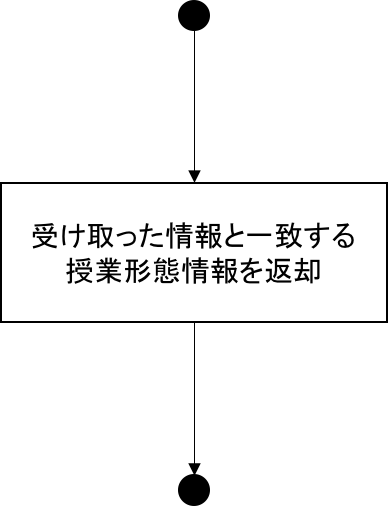
\includegraphics[width=0.8\linewidth,clip]{./img/flow/16.png}
  \end{center}
 \end{minipage}
\end{tabular}
 \caption{左:(14)のフローチャート 中:(15)のフローチャート 右:(16)のフローチャート}\label{fig:14to15to16}
\end{figure}


\begin{figure}[htbp]
  \begin{center}
    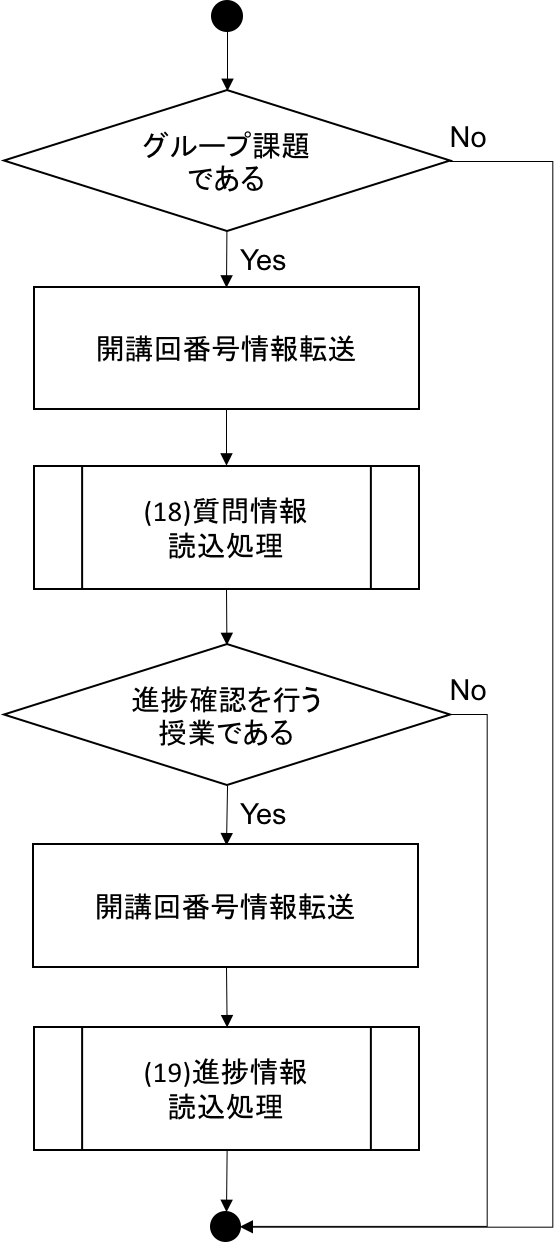
\includegraphics[width=0.35\linewidth,clip]{./img/flow/17.png}
    \caption{(17)のフローチャート}\label{fig:17}
  \end{center}
\end{figure}


\begin{figure}[htbp]
 \begin{minipage}{0.5\hsize}
  \begin{center}
   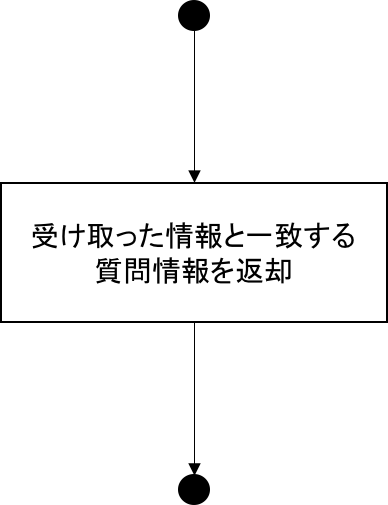
\includegraphics[width=0.5\linewidth,clip]{./img/flow/18.png}
  \end{center}
 \end{minipage}
 \begin{minipage}{0.5\hsize}
  \begin{center}
   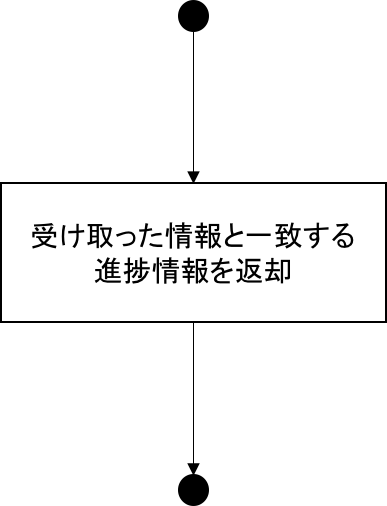
\includegraphics[width=0.5\linewidth,clip]{./img/flow/19.png}
  \end{center}
 \end{minipage}
 \caption{左:(18)のフローチャート 右:(19)のフローチャート}\label{fig:18to19}
\end{figure}

\begin{figure}[htbp]
 \begin{minipage}{0.5\hsize}
  \begin{center}
   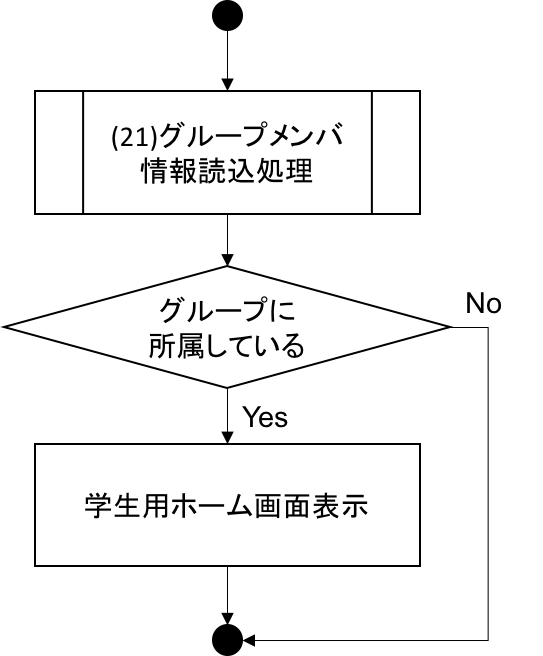
\includegraphics[width=0.75\linewidth,clip]{./img/flow/20.png}
  \end{center}
 \end{minipage}
 \begin{minipage}{0.5\hsize}
  \begin{center}
   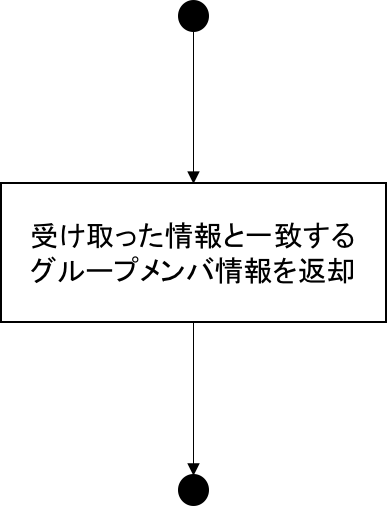
\includegraphics[width=0.5\linewidth,clip]{./img/flow/21.png}
  \end{center}
 \end{minipage}
 \caption{左:(20)のフローチャート 右:(21)のフローチャート}\label{fig:20to21}
\end{figure}

\begin{figure}[htbp]
  \begin{center}
    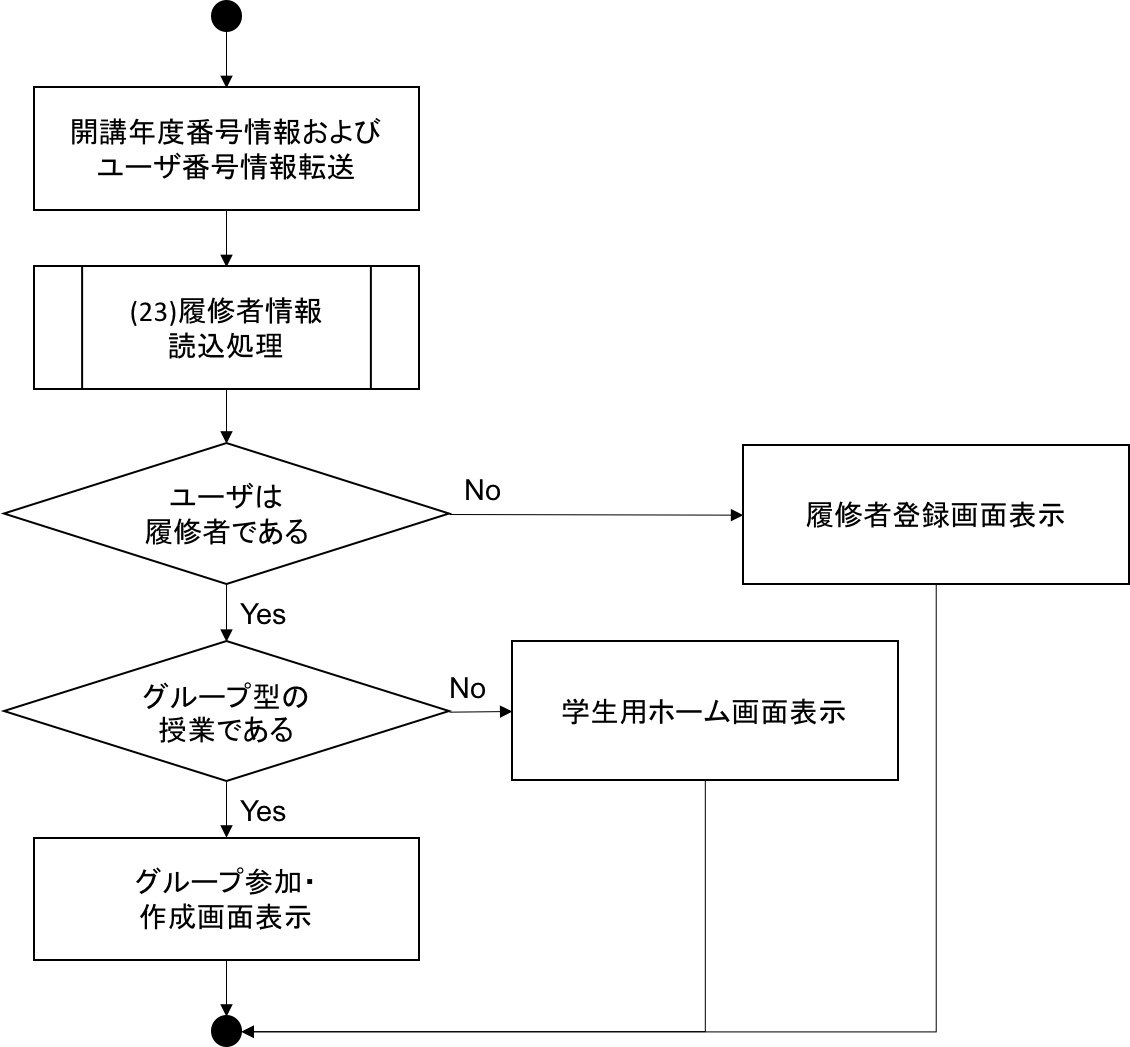
\includegraphics[width=0.75\linewidth,clip]{./img/flow/22.png}
    \caption{(22)のフローチャート}\label{fig:22}
  \end{center}
\end{figure}

\begin{figure}[htbp]
  \begin{tabular}{c}
 \begin{minipage}{0.33\hsize}
  \begin{center}
   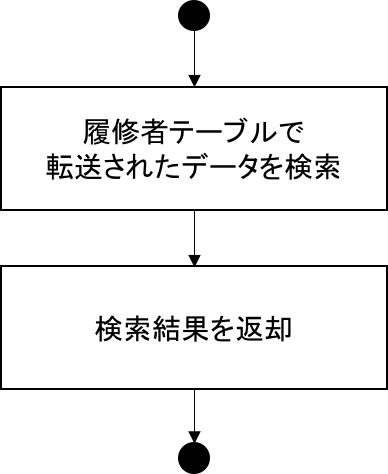
\includegraphics[width=0.8\linewidth,clip]{./img/flow/23.png}
  \end{center}
 \end{minipage}
 \begin{minipage}{0.33\hsize}
  \begin{center}
   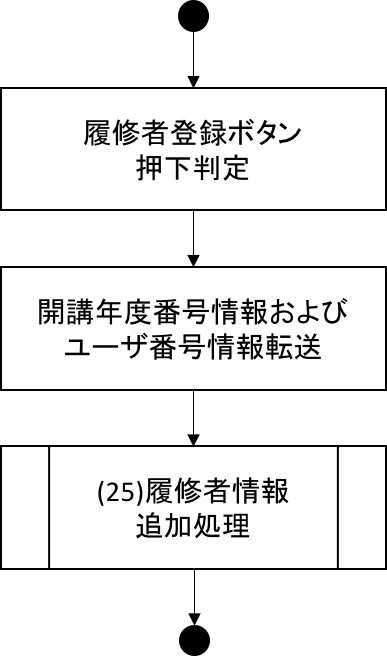
\includegraphics[width=0.8\linewidth,clip]{./img/flow/24.png}
  \end{center}
 \end{minipage}
 \begin{minipage}{0.33\hsize}
  \begin{center}
   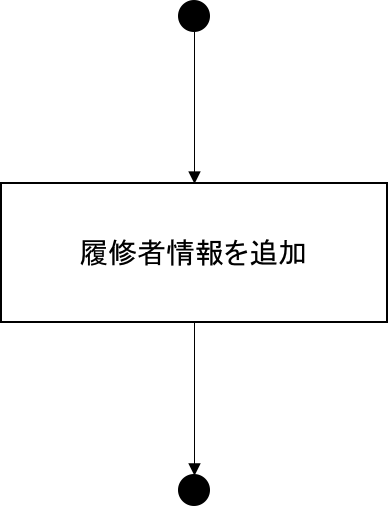
\includegraphics[width=0.8\linewidth,clip]{./img/flow/25.png}
  \end{center}
 \end{minipage}
\end{tabular}
 \caption{左:(23)のフローチャート 中:(24)のフローチャート 右:(25)のフローチャート}\label{fig:23to24to25}
\end{figure}


\clearpage


\subsection{ログインシステム(管理者用)}
ログインシステム(管理者用)では、ログイン時に権限レベルを判定し、管理者であった場合に管理者用ホーム画面へ遷移する処理が行われます。
ログインシステム(管理者用)のシーケンス図とフローチャートを以下に示します。

\begin{figure}[htbp]
  \begin{center}
    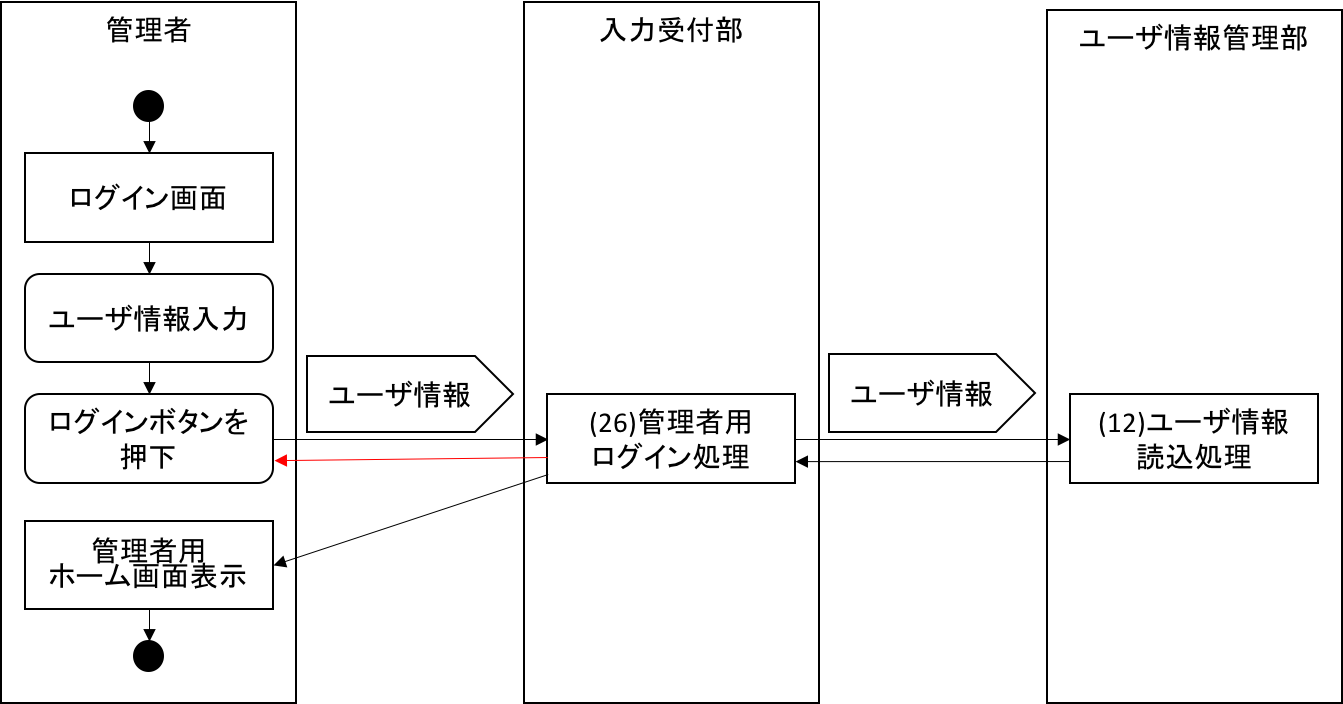
\includegraphics[width=1\linewidth,clip]{./img/seq6.png}
    \caption{ログインシステム(管理者用)のシーケンス図}\label{fig:seq6}
  \end{center}
\end{figure}

(26)は、ログインボタンを押下することで管理者用ホーム画面へ遷移する処理です。


\begin{figure}[htbp]
  \begin{center}
    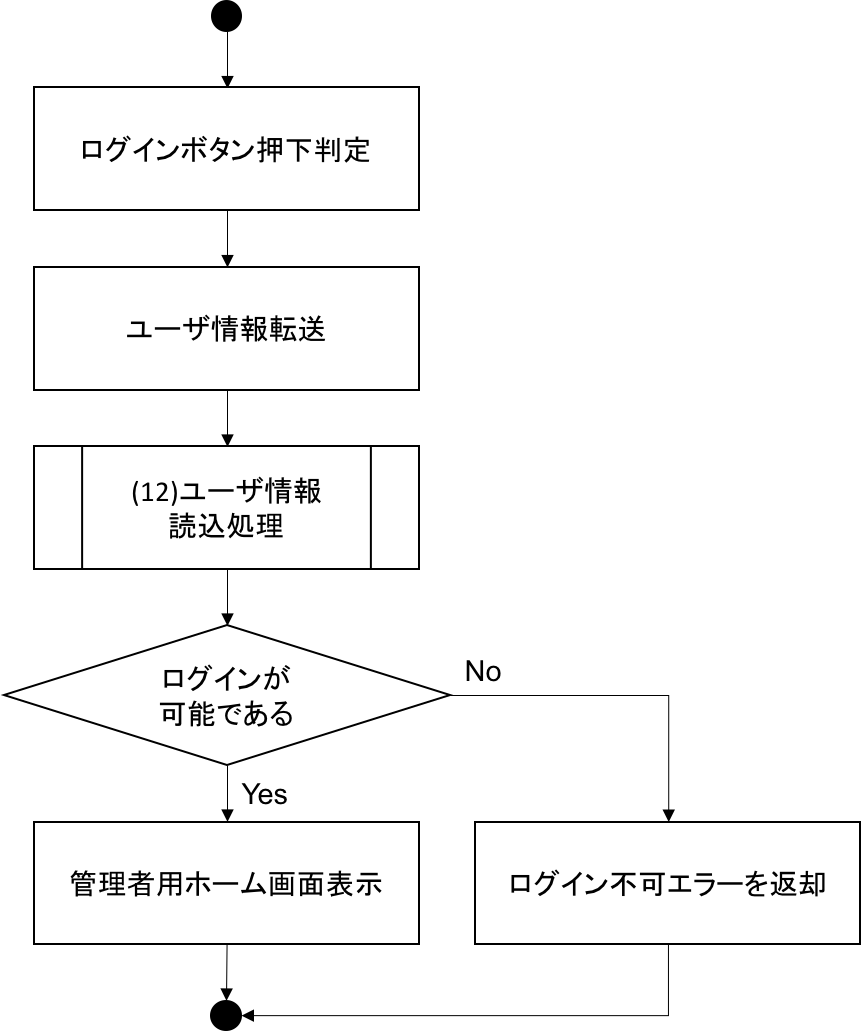
\includegraphics[width=0.55\linewidth,clip]{./img/flow/26.png}
    \caption{(26)のフローチャート}\label{fig:26}
  \end{center}
\end{figure}

\clearpage

\subsection{グループ作成システム}
グループ作成システムでは、グループ作成・参加画面にてグループ作成ボタンを押下することで処理が行われます。
グループ作成システムのシーケンス図とフローチャートを以下に示します。

\begin{figure}[htbp]
  \begin{center}
    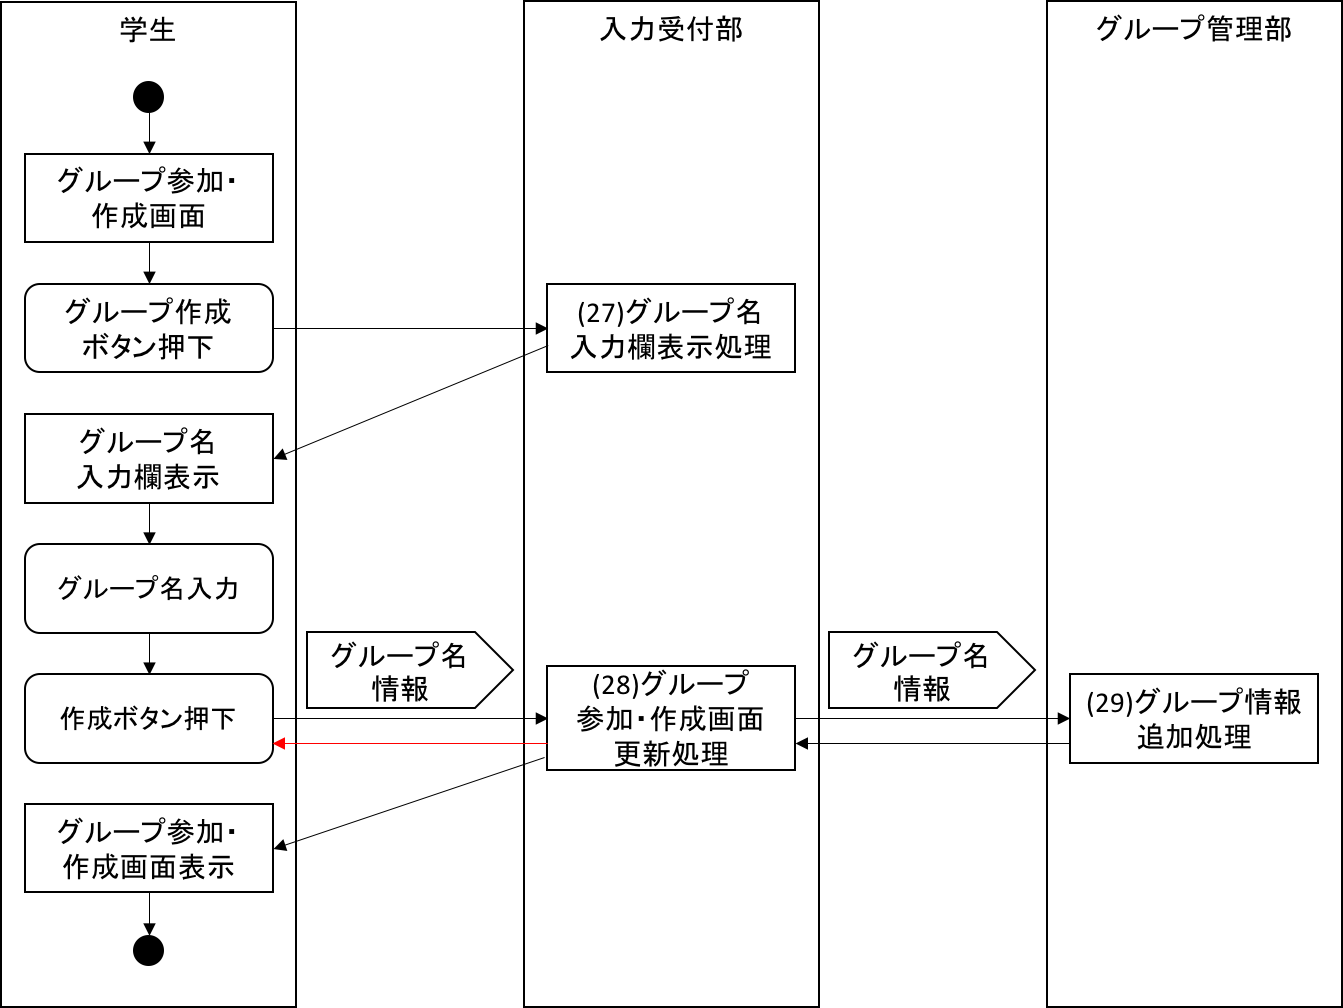
\includegraphics[width=1\linewidth,clip]{./img/seq7.png}
    \caption{グループ作成システムのシーケンス図}\label{fig:seq7}
  \end{center}
\end{figure}


(27)は、グループ作成ボタンを押下することで、新規グループを作成させるポップアップを表示する処理です。\\
(28)・(29)は、グループ名を入力した後作成ボタンを押下することで、同一グループが存在していないかの判定を行い、グループを作成する処理です。


\begin{figure}[htbp]
 \begin{minipage}{0.5\hsize}
  \begin{center}
   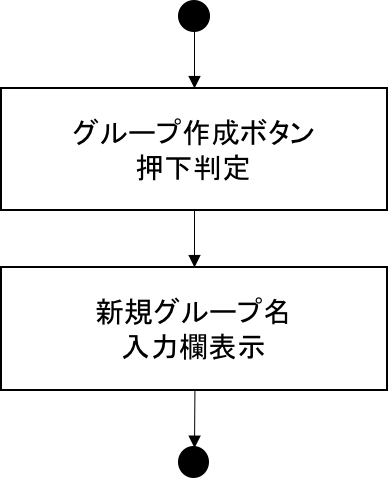
\includegraphics[width=0.5\linewidth,clip]{./img/flow/27.png}
  \end{center}
 \end{minipage}
 \begin{minipage}{0.5\hsize}
  \begin{center}
   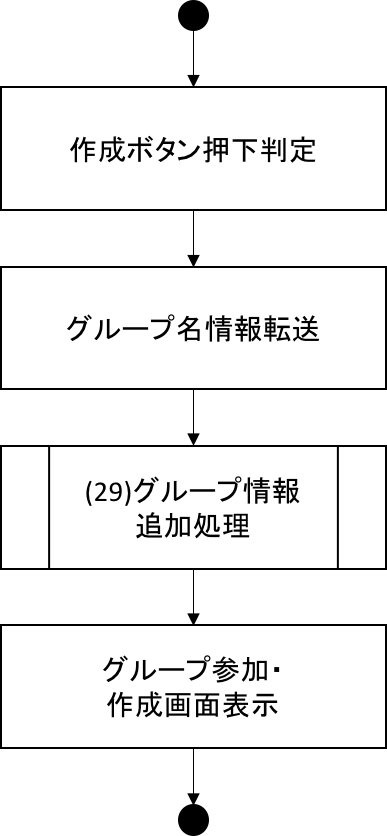
\includegraphics[width=0.5\linewidth,clip]{./img/flow/28.png}
  \end{center}
 \end{minipage}
 \caption{左:(27)のフローチャート 右:(28)のフローチャート}\label{fig:27to28}
\end{figure}

\begin{figure}[htbp]
  \begin{center}
    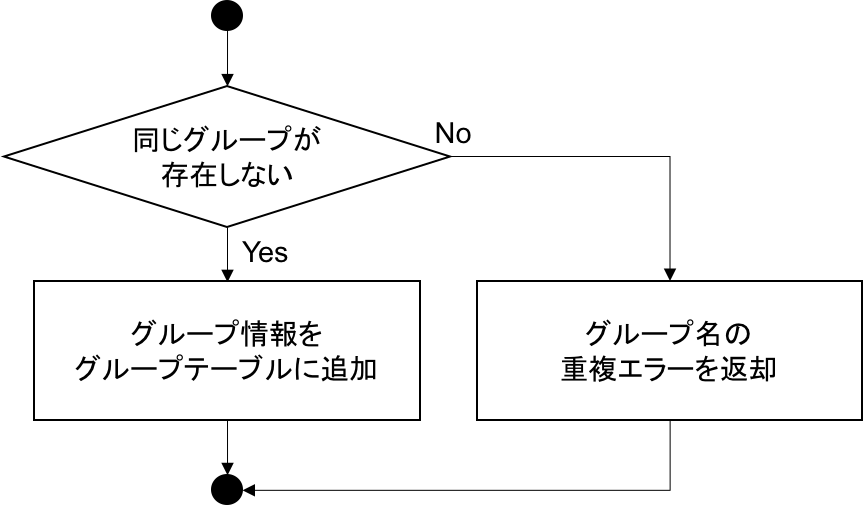
\includegraphics[width=0.75\linewidth,clip]{./img/flow/29.png}
    \caption{(29)のフローチャート}\label{fig:29}
  \end{center}
\end{figure}


\clearpage

\subsection{グループ参加システム}
グループ参加システムでは、グループ作成・参加画面においてグループボタンを押下し、該当グループの参加ボタンを押下することで処理が行われます。
グループ参加システムのシーケンス図とフローチャートを以下に示します。

\begin{figure}[htbp]
  \begin{center}
    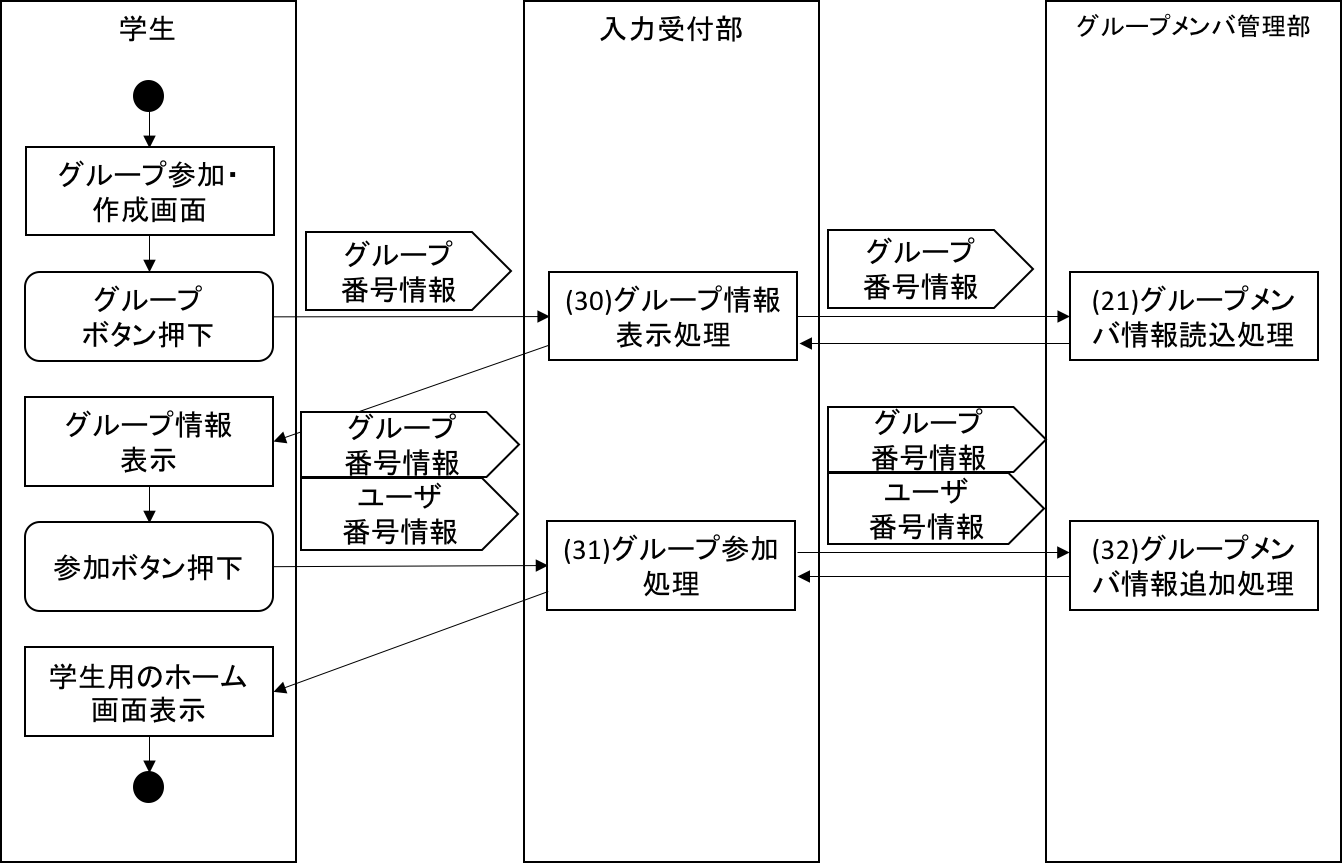
\includegraphics[width=1\linewidth,clip]{./img/seq8.png}
    \caption{グループ参加システムのシーケンス図}\label{fig:seq8}
  \end{center}
\end{figure}

(30)は、グループのボタンを押下することでグループの情報を表示する処理です。\\
(31)・(32)は、グループの参加ボタンを押下することで押下したユーザを該当グループに参加させる処理です。


\begin{figure}[htbp]
  \begin{tabular}{c}
 \begin{minipage}{0.33\hsize}
  \begin{center}
   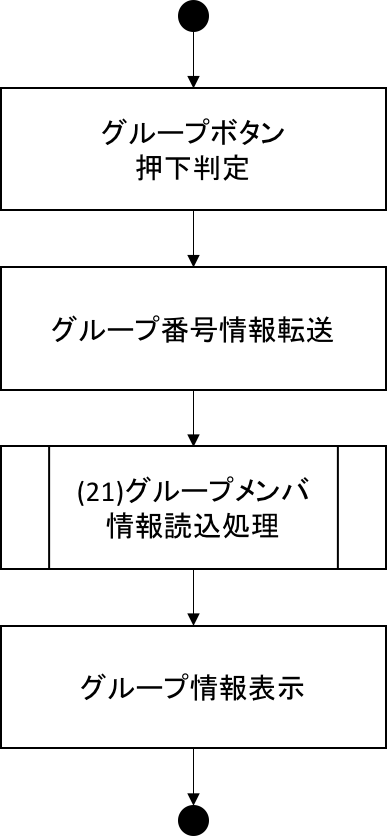
\includegraphics[width=0.8\linewidth,clip]{./img/flow/30.png}
  \end{center}
 \end{minipage}
 \begin{minipage}{0.33\hsize}
  \begin{center}
   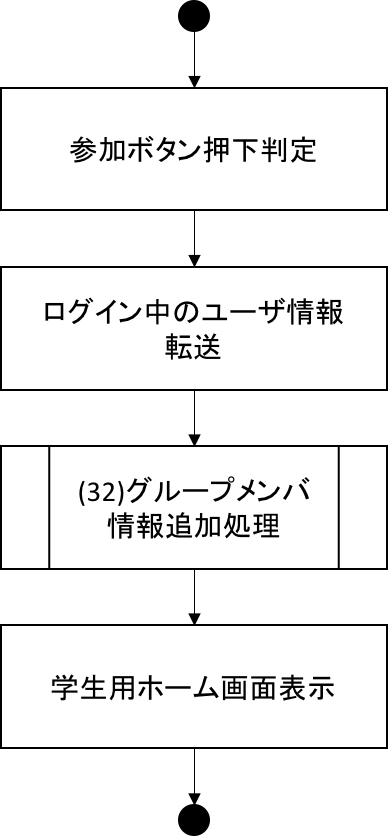
\includegraphics[width=0.8\linewidth,clip]{./img/flow/31.png}
  \end{center}
 \end{minipage}
 \begin{minipage}{0.33\hsize}
  \begin{center}
   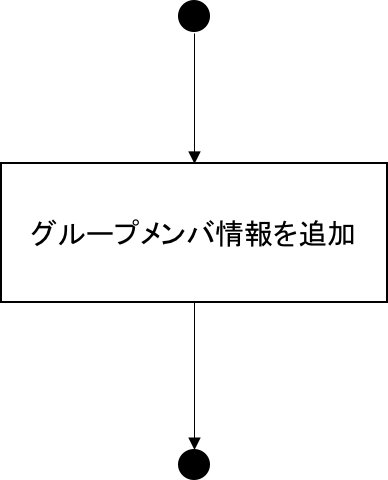
\includegraphics[width=0.8\linewidth,clip]{./img/flow/32.png}
  \end{center}
 \end{minipage}
\end{tabular}
 \caption{左:(30)のフローチャート 中:(31)のフローチャート 右:(32)のフローチャート}\label{fig:30to31to32}
\end{figure}


\clearpage



\subsection{グループ編集システム}
グループ情報編集システムでは、管理者がグループ情報編集画面において削除ボタン及び決定ボタンを押すことで処理が行われます。
グループ情報編集システムのシーケンス図とフローチャートを以下に示します。

\begin{figure}[htbp]
  \begin{center}
    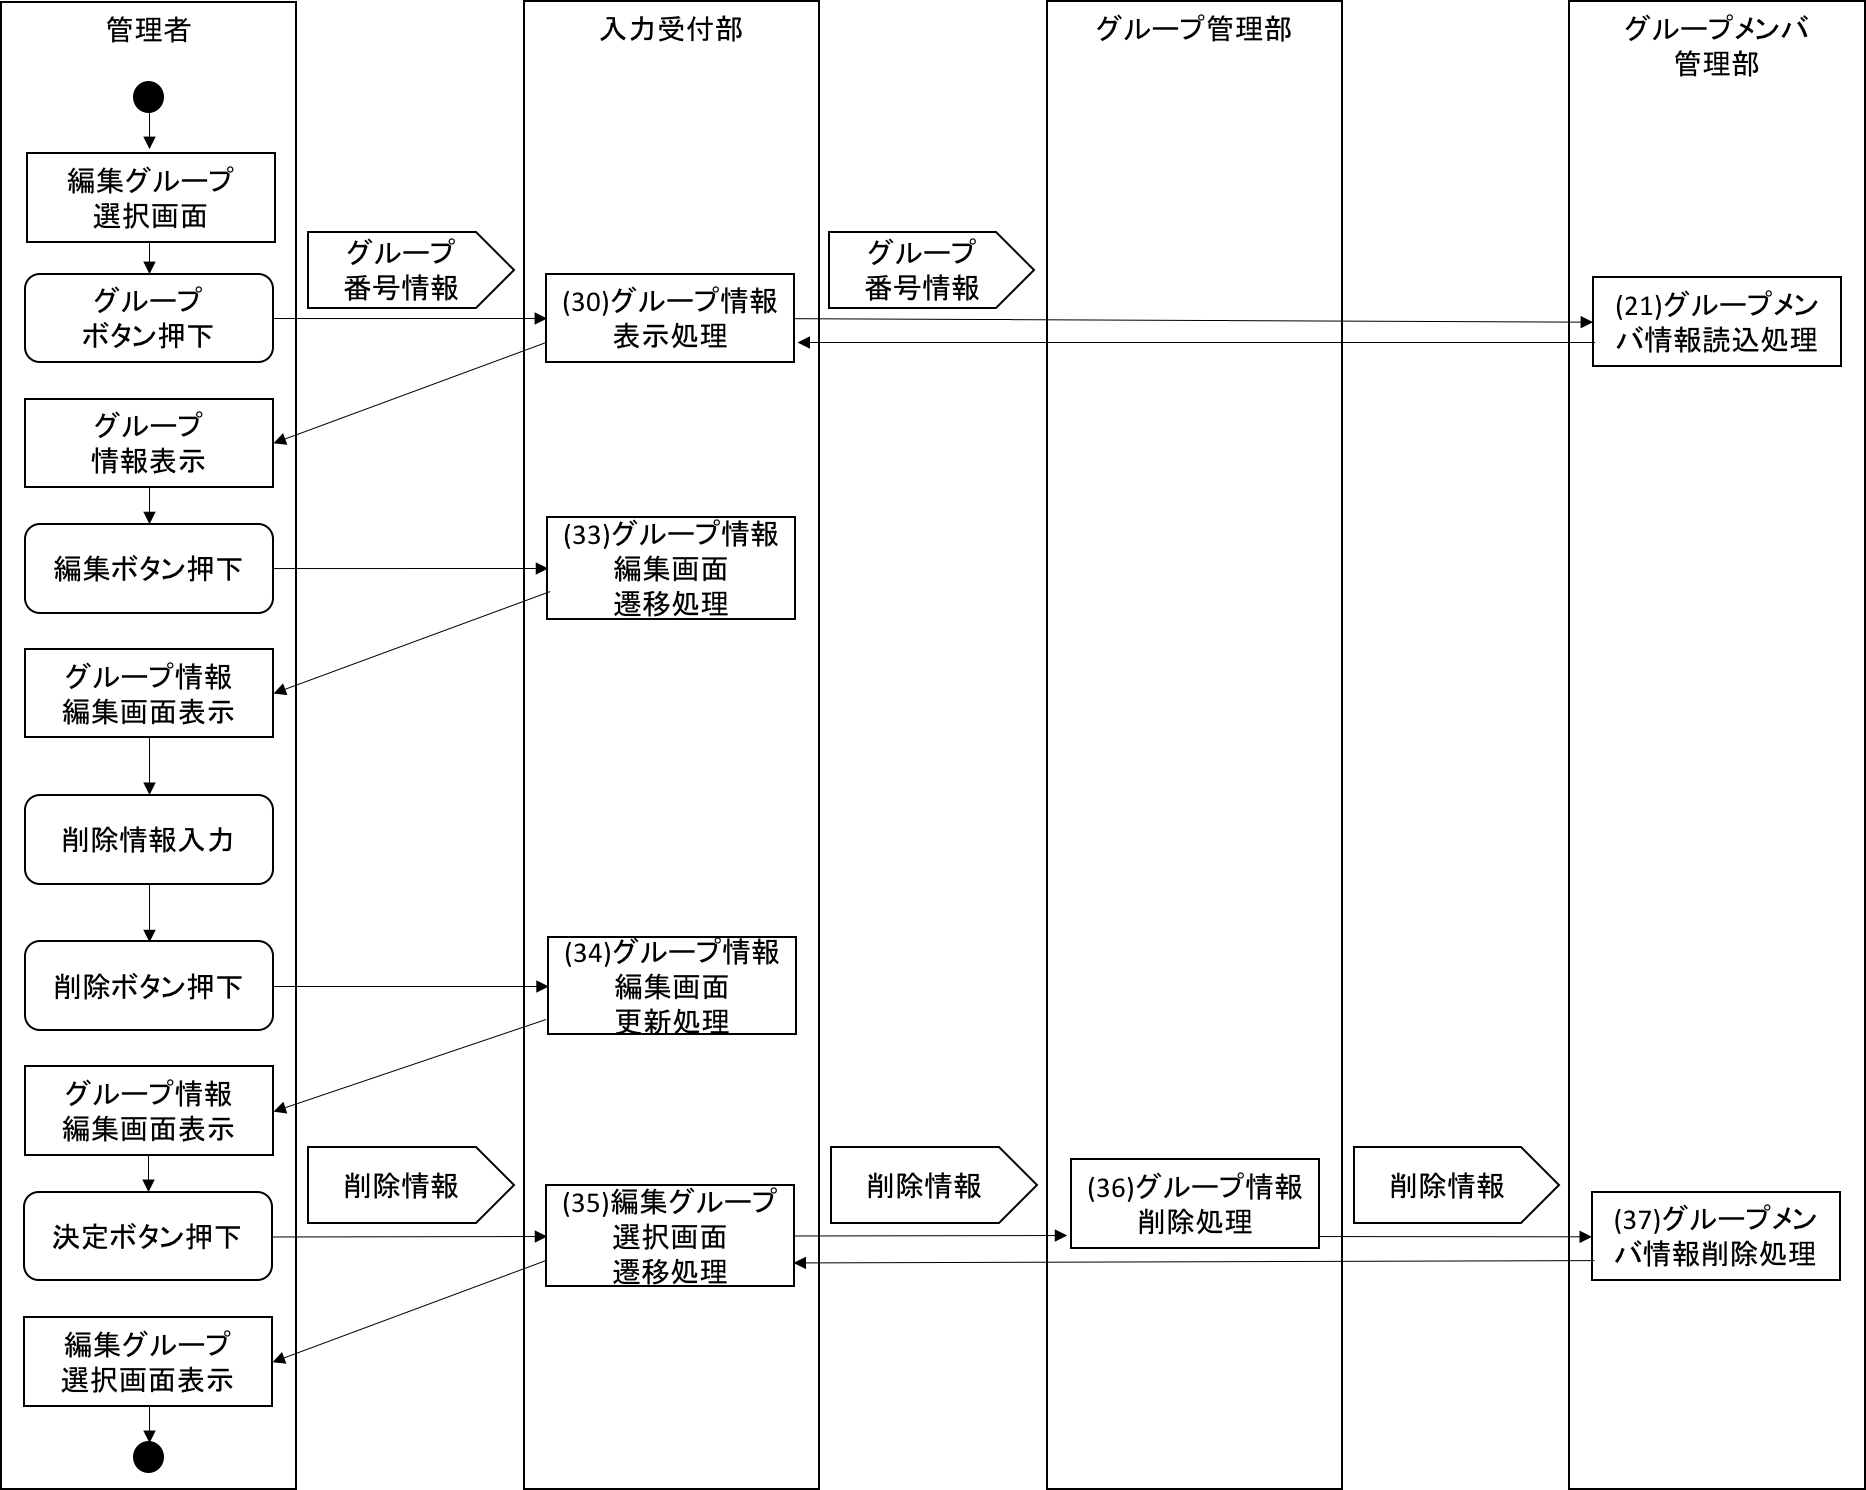
\includegraphics[width=1\linewidth,clip]{./img/seq9.png}
    \caption{グループ編集システムのシーケンス図}\label{fig:seq9}
  \end{center}
\end{figure}

(33)は、編集グループ選択画面にて編集ボタンを押下することでグループ情報編集画面へ遷移する処理です。\\
(34)は、削除ボタンを押下することで画面上で非表示にする処理です。\\
(35)~(37)は、決定ボタンを押下することで、削除ボタンにて非表示にした情報を削除する処理です。


\begin{figure}[htbp]
 \begin{minipage}{0.5\hsize}
  \begin{center}
   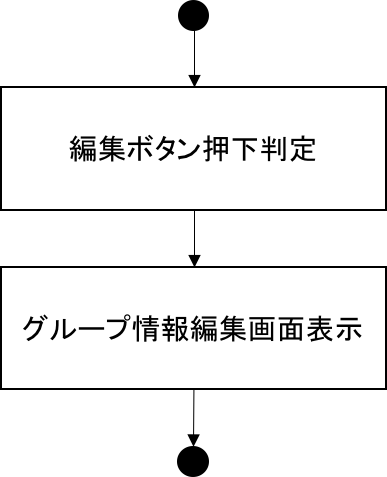
\includegraphics[width=0.6\linewidth,clip]{./img/flow/33.png}
  \end{center}
 \end{minipage}
 \begin{minipage}{0.5\hsize}
  \begin{center}
   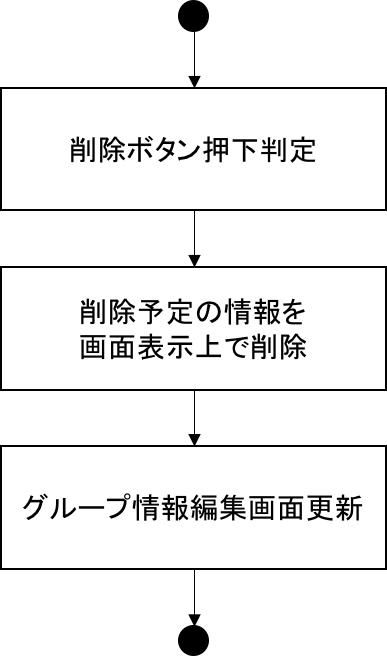
\includegraphics[width=0.6\linewidth,clip]{./img/flow/34.png}
  \end{center}
 \end{minipage}
 \caption{左:(33)のフローチャート 右:(34)のフローチャート}\label{fig:33to34to35}
\end{figure}


\begin{figure}[htbp]
 \begin{center}
  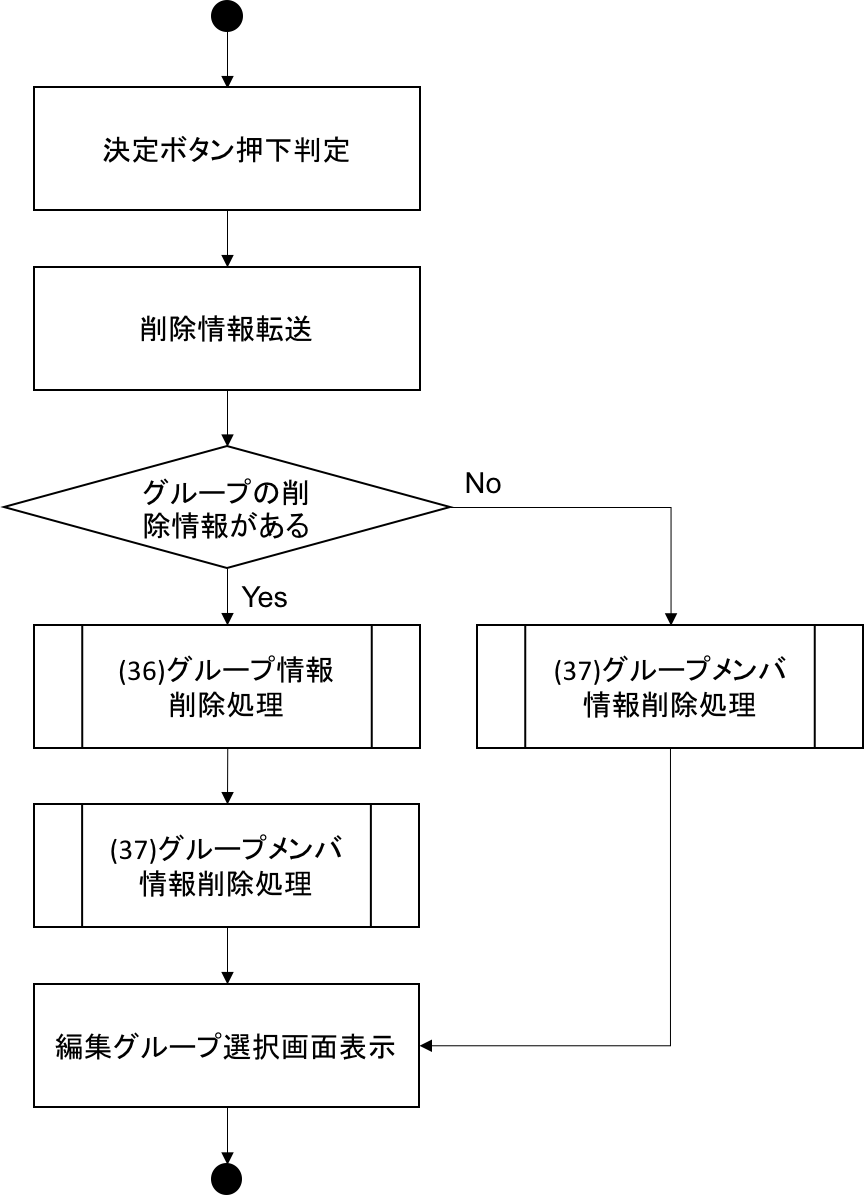
\includegraphics[width=0.5\linewidth,clip]{./img/flow/35.png}
 \end{center}
\caption{(35)のフローチャート}\label{fig:35}
\end{figure}


\begin{figure}[htbp]
 \begin{minipage}{0.5\hsize}
  \begin{center}
   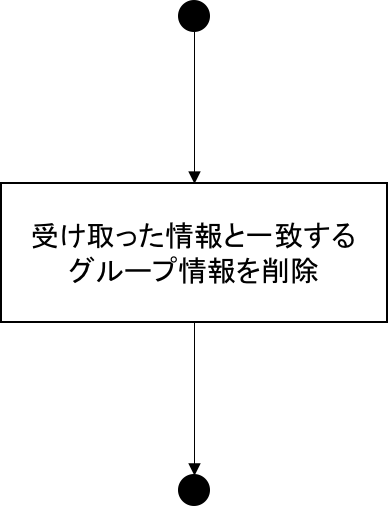
\includegraphics[width=0.6\linewidth,clip]{./img/flow/36.png}
  \end{center}
 \end{minipage}
 \begin{minipage}{0.5\hsize}
  \begin{center}
   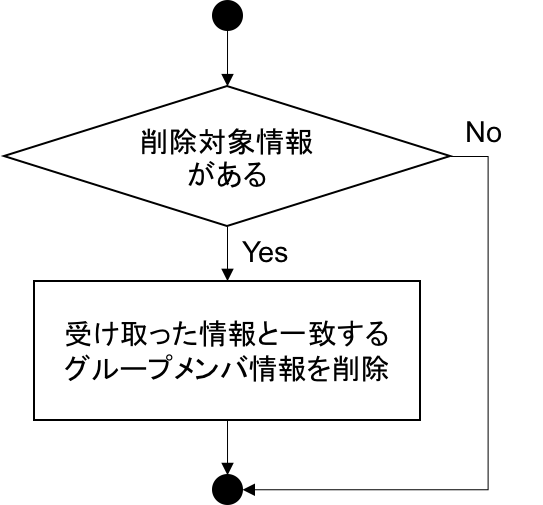
\includegraphics[width=0.7\linewidth,clip]{./img/flow/37.png}
  \end{center}
 \end{minipage}
 \caption{左:(36)のフローチャート 右:(37)のフローチャート}\label{fig:36to37}
\end{figure}

\clearpage



\subsection{クイックアクセスシステム}
クイックアクセスシステムでは、クイックアクセスが表示されている任意の画面にてクイックアクセス部分を押下することで
公開中の講義を表示する処理を行います。
クイックアクセスシステムのシーケンス図とフローチャートを以下に示します。

\begin{figure}[htbp]
  \begin{center}
    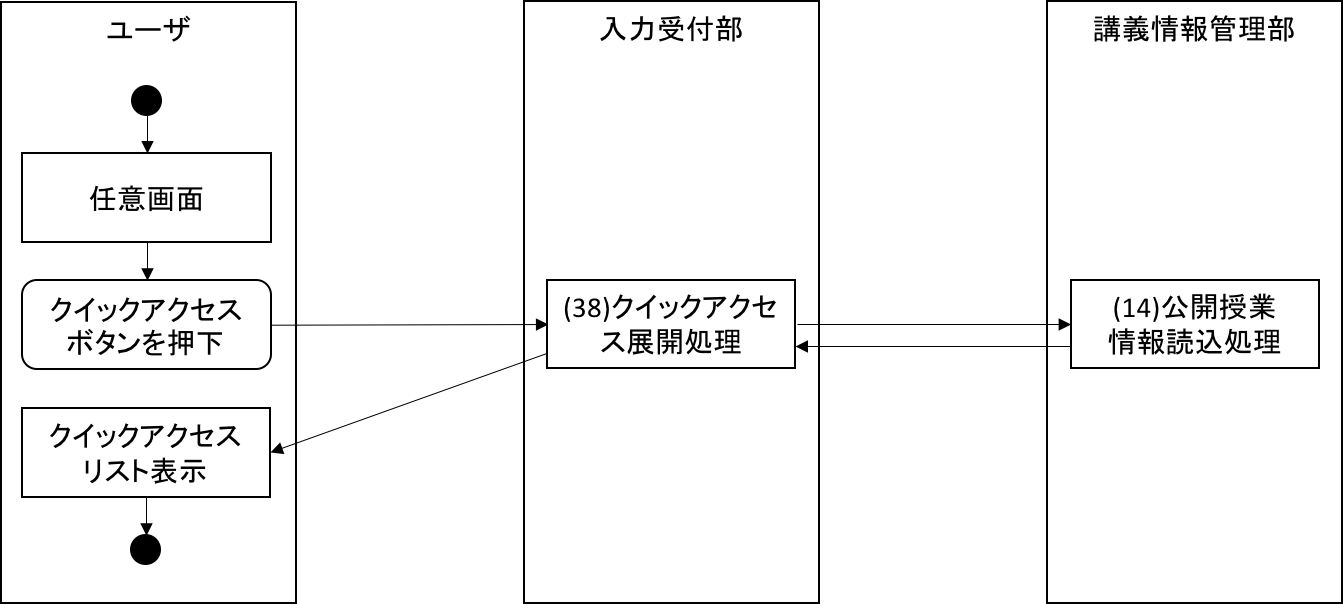
\includegraphics[width=1\linewidth,clip]{./img/seq10.png}
    \caption{クイックアクセスシステムのシーケンス図}\label{fig:seq10}
  \end{center}
\end{figure}

(38)は、クイックアクセスボタンが押下されたを判定する処理です。\\
また、押したユーザが教員であるかを判定し、開講する情報と非公開ボタンを含めて展開するか、
講義の非公開情報のみを公開するか判断します。

\begin{figure}[htbp]
  \begin{center}
    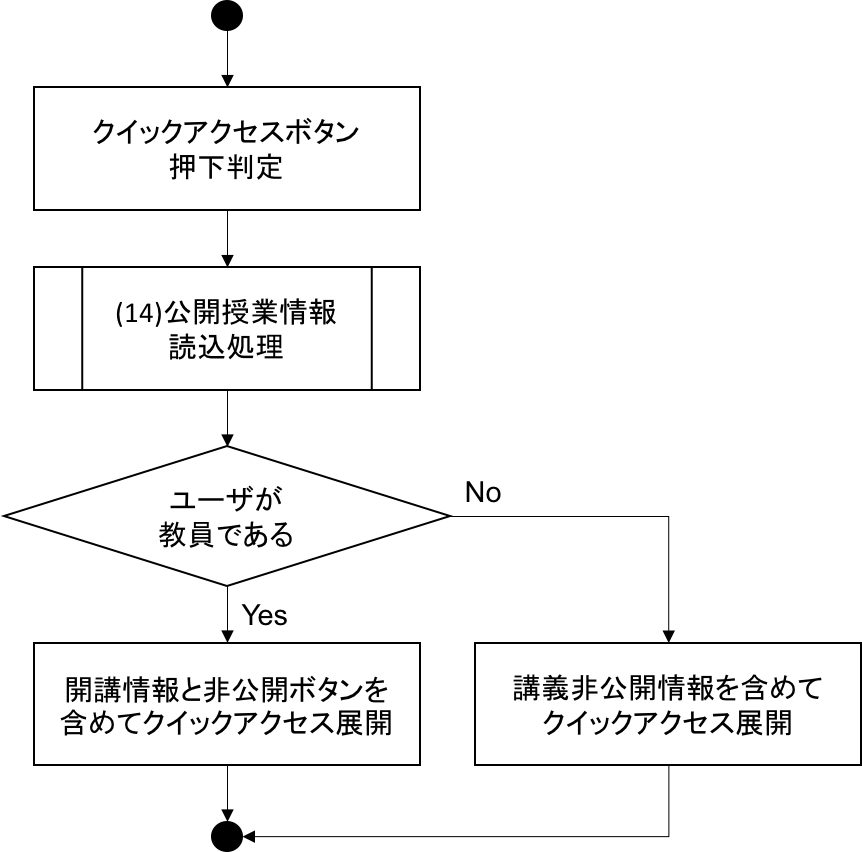
\includegraphics[width=0.5\linewidth,clip]{./img/flow/38.png}
    \caption{(38)のフローチャート}\label{fig:38}
  \end{center}
\end{figure}



\clearpage




\subsection{授業作成・編集・引継システム}
授業作成・編集・引継システムでは、授業選択画面にて各ボタンを押下することによって処理が行われます。
授業作成・編集・引継システムのシーケンス図とフローチャートを以下に示します。

\begin{figure}[htbp]
  \begin{center}
    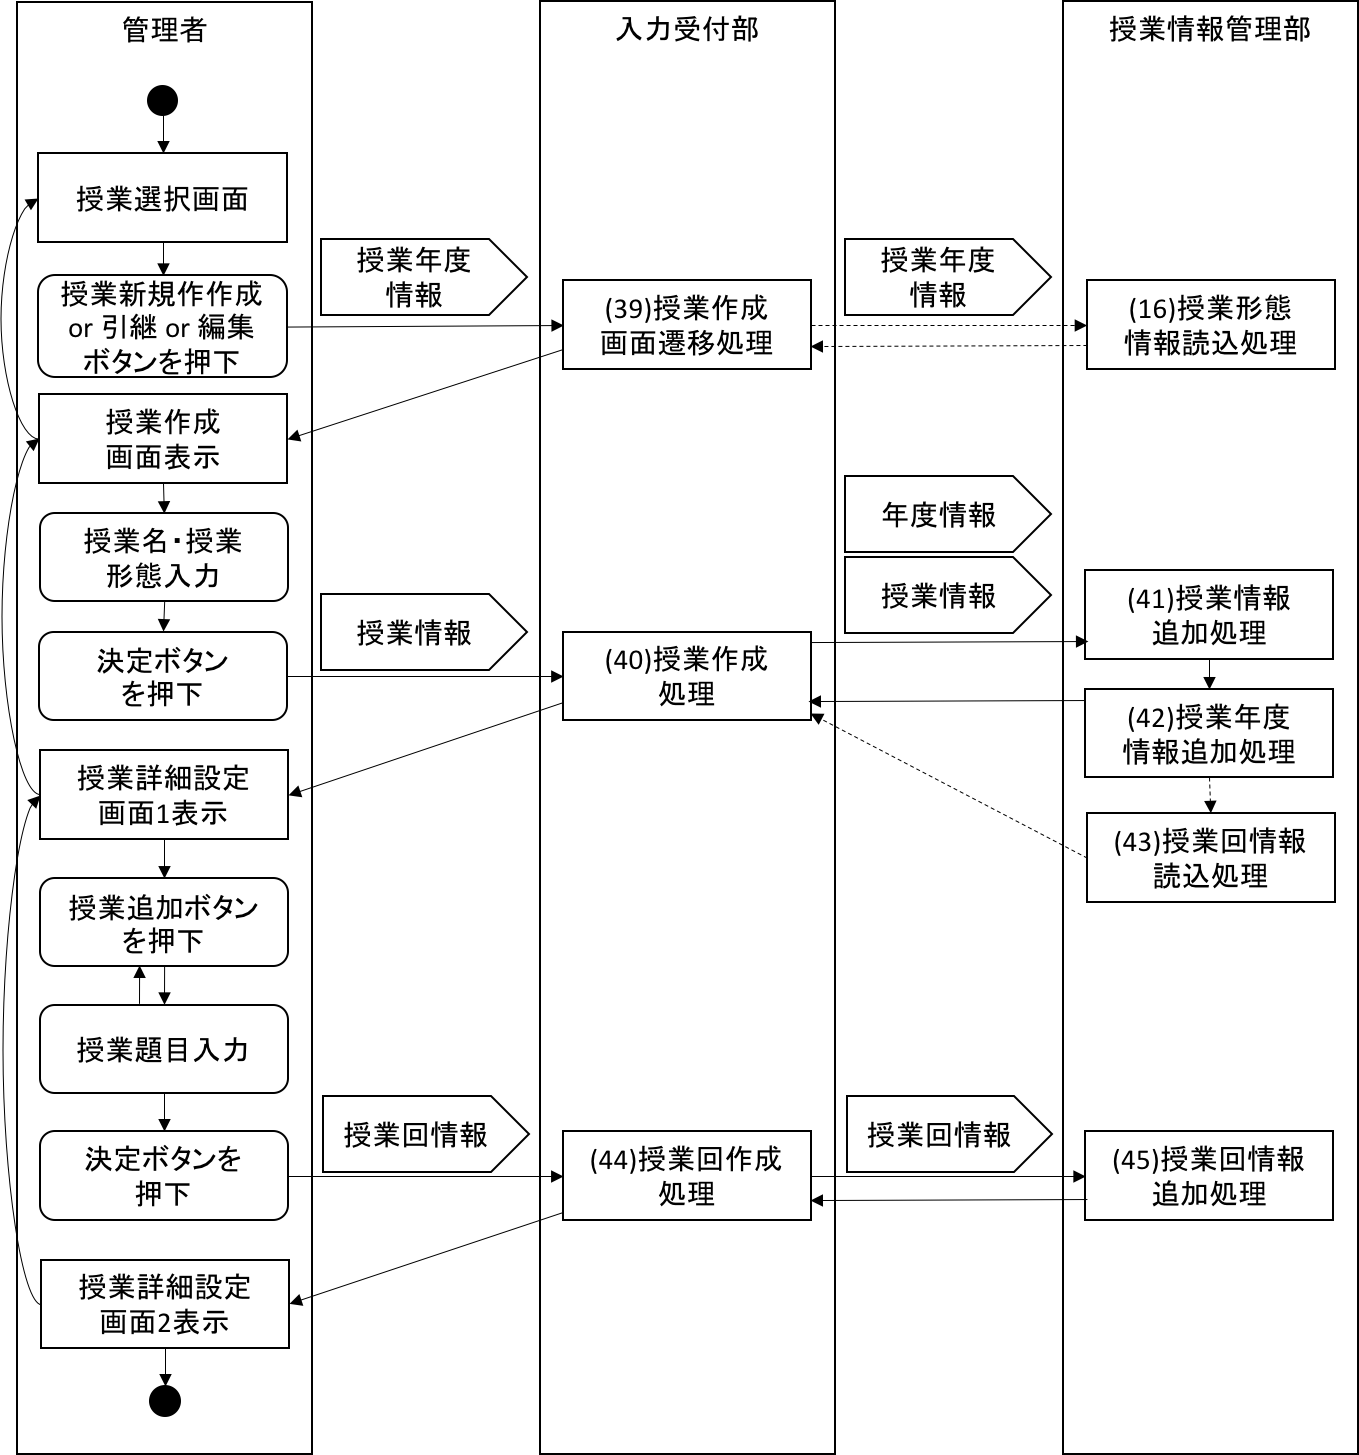
\includegraphics[width=1\linewidth,clip]{./img/seq11.png}
    \caption{授業作成・編集・引継システムのシーケンス図}\label{fig:seq11}
  \end{center}
\end{figure}

(39)は、どの作業を行うかの判定処理です。\\
(40)~(45)は、授業の作成・編集を行う処理です。

\begin{figure}[htbp]
 \begin{minipage}{0.5\hsize}
  \begin{center}
   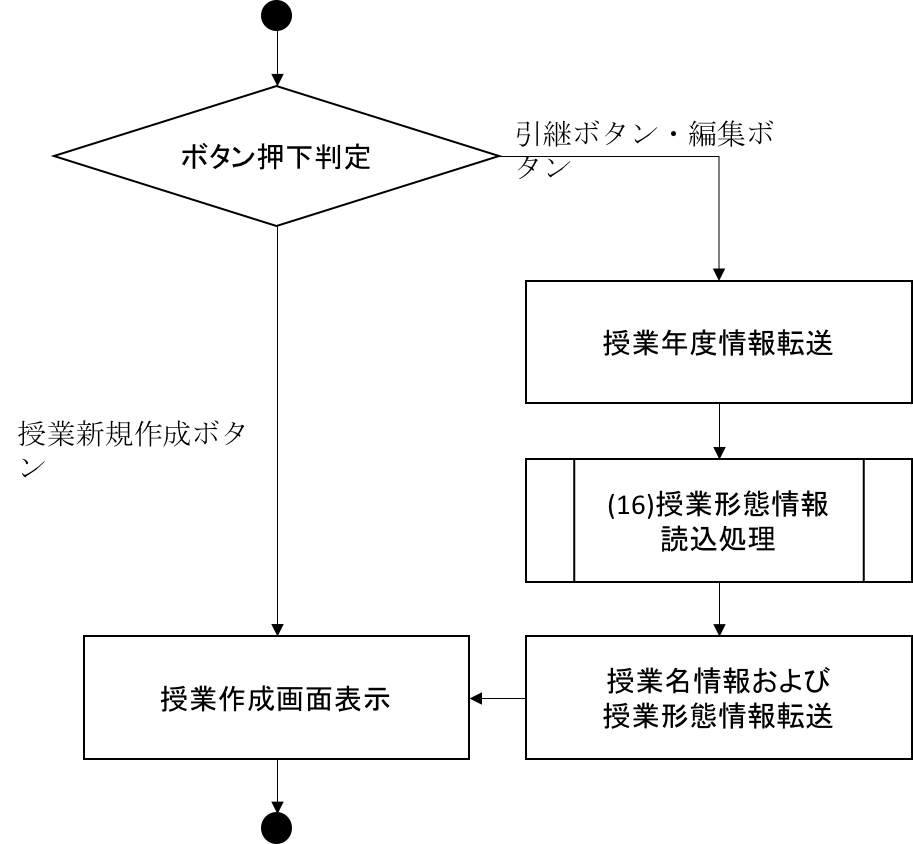
\includegraphics[width=0.9\linewidth,clip]{./img/flow/39.png}
  \end{center}
 \end{minipage}
 \begin{minipage}{0.5\hsize}
  \begin{center}
   \includegraphics[width=0.85\linewidth,clip]{./img/flow/40.png}
  \end{center}
 \end{minipage}
 \caption{左:(39)のフローチャート 右:(40)のフローチャート}\label{fig:39to40}
\end{figure}

\begin{figure}[htbp]
  \begin{tabular}{c}
 \begin{minipage}{0.33\hsize}
  \begin{center}
   \includegraphics[width=0.8\linewidth,clip]{./img/flow/41.png}
  \end{center}
 \end{minipage}
 \begin{minipage}{0.33\hsize}
  \begin{center}
   \includegraphics[width=0.8\linewidth,clip]{./img/flow/42.png}
  \end{center}
 \end{minipage}
 \begin{minipage}{0.33\hsize}
  \begin{center}
   \includegraphics[width=0.8\linewidth,clip]{./img/flow/43.png}
  \end{center}
 \end{minipage}
\end{tabular}
 \caption{左:(41)のフローチャート 中:(42)のフローチャート 右:(43)のフローチャート}\label{fig:41to42to43}
\end{figure}

\begin{figure}[htbp]
 \begin{minipage}{0.5\hsize}
  \begin{center}
   \includegraphics[width=0.5\linewidth,clip]{./img/flow/44.png}
  \end{center}
 \end{minipage}
 \begin{minipage}{0.5\hsize}
  \begin{center}
   \includegraphics[width=0.5\linewidth,clip]{./img/flow/45.png}
  \end{center}
 \end{minipage}
 \caption{左:(44)のフローチャート 右:(45)のフローチャート}\label{fig:44to45}
\end{figure}


\clearpage



\subsection{課題作成システム}
課題作成システムでは、授業詳細設定画面3にて課題追加ボタンを押下し、課題名と内容を入力し決定ボタンを押下することによって処理が行われます。
課題作成システムのシーケンス図とフローチャートを以下に示します。

\begin{figure}[htbp]
  \begin{center}
    \includegraphics[width=1\linewidth,clip]{./img/seq12.png}
    \caption{課題作成システムのシーケンス図}\label{fig:seq12}
  \end{center}
\end{figure}

(46)は、授業詳細設定画面3へ遷移する処理です。\\
(47)・(48)は、課題を作成する処理です。

\begin{figure}[htbp]
  \begin{tabular}{c}
 \begin{minipage}{0.33\hsize}
  \begin{center}
   \includegraphics[width=0.8\linewidth,clip]{./img/flow/46.png}
  \end{center}
 \end{minipage}
 \begin{minipage}{0.33\hsize}
  \begin{center}
   \includegraphics[width=0.8\linewidth,clip]{./img/flow/47.png}
  \end{center}
 \end{minipage}
 \begin{minipage}{0.33\hsize}
  \begin{center}
   \includegraphics[width=0.8\linewidth,clip]{./img/flow/48.png}
  \end{center}
 \end{minipage}
\end{tabular}
 \caption{左:(46)のフローチャート 中:(47)のフローチャート 右:(48)のフローチャート}\label{fig:46to47to48}
\end{figure}
\clearpage




\subsection{授業公開・非公開システム}
授業公開・非公開システムは、授業回選択画面にて公開ボタンを押すことで授業が学生に公開され、クイックアクセスに存在する非公開ボタンにて学生への公開を終了する処理を行います。
授業公開・非公開システムのシーケンス図とフローチャートを以下に示します。

\begin{figure}[htbp]
  \begin{center}
    \includegraphics[width=1\linewidth,clip]{./img/seq13.png}
    \caption{授業公開・非公開システムのシーケンス図}\label{fig:seq13}
  \end{center}
\end{figure}


(49)~(52)は、授業の公開を行う処理です。\\
(53)~(56)は、授業を非公開にする処理です。

\begin{figure}[htbp]
 \begin{minipage}{0.5\hsize}
  \begin{center}
   \includegraphics[width=0.5\linewidth,clip]{./img/flow/49.png}
  \end{center}
 \end{minipage}
 \begin{minipage}{0.5\hsize}
  \begin{center}
   \includegraphics[width=0.8\linewidth,clip]{./img/flow/50.png}
  \end{center}
 \end{minipage}
 \caption{左:(49)のフローチャート 右:(50)のフローチャート}\label{fig:49to50}
\end{figure}

\begin{figure}[htbp]
  \begin{tabular}{c}
 \begin{minipage}{0.33\hsize}
  \begin{center}
   \includegraphics[width=0.8\linewidth,clip]{./img/flow/51.png}
  \end{center}
 \end{minipage}
 \begin{minipage}{0.33\hsize}
  \begin{center}
   \includegraphics[width=0.8\linewidth,clip]{./img/flow/52.png}
  \end{center}
 \end{minipage}
 \begin{minipage}{0.33\hsize}
  \begin{center}
   \includegraphics[width=0.8\linewidth,clip]{./img/flow/53.png}
  \end{center}
 \end{minipage}
\end{tabular}
 \caption{左:(51)のフローチャート 中:(52)のフローチャート 右:(53)のフローチャート}\label{fig:51to52to53}
\end{figure}

\begin{figure}[htbp]
  \begin{center}
   \includegraphics[width=0.5\linewidth,clip]{./img/flow/54.png}
  \end{center}
 \caption{(54)のフローチャート}\label{fig:54}
\end{figure}

\begin{figure}[htbp]
 \begin{minipage}{0.5\hsize}
  \begin{center}
   \includegraphics[width=0.6\linewidth,clip]{./img/flow/55.png}
  \end{center}
 \end{minipage}
 \begin{minipage}{0.5\hsize}
  \begin{center}
   \includegraphics[width=0.6\linewidth,clip]{./img/flow/56.png}
  \end{center}
 \end{minipage}
 \caption{左:(55)のフローチャート 右:(56)のフローチャート}\label{fig:54to55to56}
\end{figure}

\clearpage



\subsection{進捗確認システム}
進捗確認システムでは、授業回を選択し、授業作成時に設定した授業形態に応じて、学生の課題の進捗状況を表示する処理が行われます。
この進捗確認システムのシーケンス図とフローチャートを以下に示します。

\begin{figure}[htbp]
  \begin{center}
    \includegraphics[width=1\linewidth,clip]{./img/seq14.png}
    \caption{進捗確認システムのシーケンス図}\label{fig:seq14}
  \end{center}
\end{figure}

(57)・(58)は、進捗を確認する授業がグループワークかどうかの判定を行う処理です。\\
(59)は、課題の進捗の更新を行う処理です。

\begin{figure}[htbp]
  \begin{tabular}{c}
 \begin{minipage}{0.33\hsize}
  \begin{center}
   \includegraphics[width=0.8\linewidth,clip]{./img/flow/57.png}
  \end{center}
 \end{minipage}
 \begin{minipage}{0.33\hsize}
  \begin{center}
   \includegraphics[width=0.8\linewidth,clip]{./img/flow/58.png}
  \end{center}
 \end{minipage}
 \begin{minipage}{0.33\hsize}
  \begin{center}
   \includegraphics[width=0.8\linewidth,clip]{./img/flow/59.png}
  \end{center}
 \end{minipage}
\end{tabular}
 \caption{左:(57)のフローチャート 中:(58)のフローチャート 右:(59)のフローチャート}\label{fig:57to58to59}
\end{figure}


\clearpage




\subsection{進捗送信システム}
進捗送信システムでは、学生が(学生用←いらないと思う)ホーム画面において進捗状況を入力し、更新ボタンを押下することによって処理が行われます。
進捗送信システムのシーケンス図とフローチャートを以下に示します。

\begin{figure}[htbp]
  \begin{center}
    \includegraphics[width=1\linewidth,clip]{./img/seq15.png}
    \caption{進捗送信システムのシーケンス図}\label{fig:seq15}
  \end{center}
\end{figure}

(60)・(61)は進捗情報をデータベースに追加する処理です。


\begin{figure}[htbp]
 \begin{minipage}{0.5\hsize}
  \begin{center}
   \includegraphics[width=0.5\linewidth,clip]{./img/flow/60.png}
  \end{center}
 \end{minipage}
 \begin{minipage}{0.5\hsize}
  \begin{center}
   \includegraphics[width=0.5\linewidth,clip]{./img/flow/61.png}
  \end{center}
 \end{minipage}
 \caption{左:(60)のフローチャート 右:(61)のフローチャート}\label{fig:60to61}
\end{figure}


\clearpage


\subsection{質問閲覧システム}
質問閲覧システムでは、学生がログインすることによって現在公開されている授業の質問を表示する処理です。
質問閲覧システムのシーケンス図とフローチャートを以下に示します。


\begin{figure}[htbp]
  \begin{center}
    \includegraphics[width=1\linewidth,clip]{./img/seq16.png}
    \caption{質問閲覧システムのシーケンス図}\label{fig:seq16}
  \end{center}
\end{figure}

(62)は、学生用ホーム画面に遷移する処理です。\\
(63)・(64)は、学生の進捗状況を読み込む処理です。

\begin{figure}[htbp]
  \begin{center}
   \includegraphics[width=0.5\linewidth,clip]{./img/flow/62.png}
  \end{center}
 \caption{(62)のフローチャート}\label{fig:62}
\end{figure}

\begin{figure}[htbp]
 \begin{minipage}{0.5\hsize}
  \begin{center}
   \includegraphics[width=0.6\linewidth,clip]{./img/flow/63.png}
  \end{center}
 \end{minipage}
 \begin{minipage}{0.5\hsize}
  \begin{center}
   \includegraphics[width=0.6\linewidth,clip]{./img/flow/64.png}
  \end{center}
 \end{minipage}
 \caption{左:(63)のフローチャート 右:(64)のフローチャート}\label{fig:62to63to64}
\end{figure}

\clearpage



\subsection{過去の質問閲覧システム}
過去の質問閲覧システムでは、学生が過去に行われた授業を選択することによって表示処理が行われます。
過去の質問閲覧システムのシーケンス図とフローチャートを以下に示します。

\begin{figure}[htbp]
  \begin{center}
    \includegraphics[width=1\linewidth,clip]{./img/seq17.png}
    \caption{過去の質問閲覧システムのシーケンス図}\label{fig:seq17}
  \end{center}
\end{figure}

(65)~(67)は、対応する授業の過去の質問を表示する処理です。

\begin{figure}[htbp]
 \begin{minipage}{0.5\hsize}
  \begin{center}
   \includegraphics[width=0.4\linewidth,clip]{./img/flow/65.png}
  \end{center}
 \end{minipage}
 \begin{minipage}{0.5\hsize}
  \begin{center}
   \includegraphics[width=0.4\linewidth,clip]{./img/flow/66.png}
  \end{center}
 \end{minipage}

 \caption{左:(65)のフローチャート 右:(66)のフローチャート}\label{fig:65to66to67}
\end{figure}

\begin{figure}[htbp]
\begin{center}
 \includegraphics[width=0.5\linewidth,clip]{./img/flow/67.png}
\end{center}
 \caption{(67)のフローチャート}\label{fig:67}
\end{figure}

\clearpage




\subsection{質問送信システム}
質問送信システムでは、質問画面にて質問を入力し、質問分類ボタンを押下することによって処理が行われます。
質問送信システムのシーケンス図とフローチャートを以下に示します。

\begin{figure}[htbp]
  \begin{center}
    \includegraphics[width=1\linewidth,clip]{./img/seq18.png}
    \caption{質問送信システムのシーケンス図}\label{fig:seq18}
  \end{center}
\end{figure}

(68)は、質問画面へ遷移する処理です。\\
(69)~(71)は、入力した質問を送信する処理です。

\begin{figure}[htbp]
 \begin{minipage}{0.5\hsize}
  \begin{center}
   \includegraphics[width=0.5\linewidth,clip]{./img/flow/68.png}
  \end{center}
 \end{minipage}
 \begin{minipage}{0.5\hsize}
  \begin{center}
   \includegraphics[width=0.5\linewidth,clip]{./img/flow/69.png}
  \end{center}
 \end{minipage}
 \caption{左:(68)のフローチャート 右:(69)のフローチャート}\label{fig:68to69}
\end{figure}


\begin{figure}[htbp]
 \begin{minipage}{0.5\hsize}
  \begin{center}
   \includegraphics[width=0.85\linewidth,clip]{./img/flow/70.png}
  \end{center}
 \end{minipage}
 \begin{minipage}{0.5\hsize}
  \begin{center}
   \includegraphics[width=0.5\linewidth,clip]{./img/flow/71.png}
  \end{center}
 \end{minipage}
 \caption{左:(70)のフローチャート 右:(71)のフローチャート}\label{fig:70to71}
\end{figure}


\clearpage





\subsection{質問回答システム}
質問回答システムでは、管理者が質問回答画面にて回答情報を入力し、回答ボタンを押下することによって処理が行われます。
質問回答システムのシーケンス図とフローチャートを以下に示します。

\begin{figure}[htbp]
  \begin{center}
    \includegraphics[width=1\linewidth,clip]{./img/seq19.png}
    \caption{質問回答システムのシーケンス図}\label{fig:seq19}
  \end{center}
\end{figure}

(72)は、質問回答画面へ遷移する処理です。\\
(73)・(74)は、質問を回答する処理です。

\begin{figure}[htbp]
 \begin{minipage}{0.5\hsize}
  \begin{center}
   \includegraphics[width=0.9\linewidth,clip]{./img/flow/72.png}
  \end{center}
 \end{minipage}
 \begin{minipage}{0.5\hsize}
  \begin{center}
   \includegraphics[width=0.9\linewidth,clip]{./img/flow/73.png}
  \end{center}
 \end{minipage}
 \caption{左:(72)のフローチャート 右:(73)のフローチャート}\label{fig:72to73}
\end{figure}


\begin{figure}[htbp]
  \begin{center}
    \includegraphics[width=0.8\linewidth,clip]{./img/flow/74.png}
    \caption{(74)のフローチャート}\label{fig:74}
  \end{center}
\end{figure}

\clearpage

\subsection{質問編集システム}
質問編集システムでは、管理者用授業回選択画面よりどの授業に対する質問の閲覧・編集を行うかを選択することによって編集画面へ遷移することができます。
その画面上に表示されている質問に対して直接編集を行うことで、処理が行われます。
質問編集システムのシーケンス図とフローチャートを以下に示します。

\begin{figure}[htbp]
  \begin{center}
    \includegraphics[width=1\linewidth,clip]{./img/seq20.png}
    \caption{質問編集システムのシーケンス図}\label{fig:seq20}
  \end{center}
\end{figure}

(75)~(77)は、質問編集画面までの遷移を行う処理です。\\
(78)は、質問の編集を行う処理です。

\begin{figure}[htbp]
 \begin{minipage}{0.5\hsize}
  \begin{center}
   \includegraphics[width=0.5\linewidth,clip]{./img/flow/75.png}
  \end{center}
 \end{minipage}
 \begin{minipage}{0.5\hsize}
  \begin{center}
   \includegraphics[width=0.5\linewidth,clip]{./img/flow/76.png}
  \end{center}
 \end{minipage}
 \caption{左:(75)のフローチャート 右:(76)のフローチャート}\label{fig:75to76}
\end{figure}

\begin{figure}[htbp]
  \begin{center}
    \includegraphics[width=0.5\linewidth,clip]{./img/flow/77.png}
    \caption{(77)のフローチャート}\label{fig:77}
  \end{center}
\end{figure}

\clearpage

\subsection{質問削除システム}
質問削除システムでは、管理者が質問・閲覧編集画面にて削除ボタンを押下することで処理が行われます。
質問削除システムのシーケンス図とフローチャートを以下に示します。



\begin{figure}[htbp]
  \begin{center}
    \includegraphics[width=1\linewidth,clip]{./img/seq21.png}
    \caption{質問削除システムのシーケンス図}\label{fig:seq21}
  \end{center}
\end{figure}

(79)・(80)は、質問の削除を行う処理です。

\begin{figure}[htbp]
 \begin{minipage}{0.5\hsize}
  \begin{center}
   \includegraphics[width=0.5\linewidth,clip]{./img/flow/79.png}
  \end{center}
 \end{minipage}
 \begin{minipage}{0.5\hsize}
  \begin{center}
   \includegraphics[width=0.5\linewidth,clip]{./img/flow/80.png}
  \end{center}
 \end{minipage}
 \caption{左:(79)のフローチャート 右:(80)のフローチャート}\label{fig:79to80}
\end{figure}
